% Options for packages loaded elsewhere
% Options for packages loaded elsewhere
\PassOptionsToPackage{unicode}{hyperref}
\PassOptionsToPackage{hyphens}{url}
\PassOptionsToPackage{dvipsnames,svgnames,x11names}{xcolor}
%
\documentclass[
  letterpaper,
  DIV=11,
  numbers=noendperiod]{scrreprt}
\usepackage{xcolor}
\usepackage{amsmath,amssymb}
\setcounter{secnumdepth}{5}
\usepackage{iftex}
\ifPDFTeX
  \usepackage[T1]{fontenc}
  \usepackage[utf8]{inputenc}
  \usepackage{textcomp} % provide euro and other symbols
\else % if luatex or xetex
  \usepackage{unicode-math} % this also loads fontspec
  \defaultfontfeatures{Scale=MatchLowercase}
  \defaultfontfeatures[\rmfamily]{Ligatures=TeX,Scale=1}
\fi
\usepackage{lmodern}
\ifPDFTeX\else
  % xetex/luatex font selection
\fi
% Use upquote if available, for straight quotes in verbatim environments
\IfFileExists{upquote.sty}{\usepackage{upquote}}{}
\IfFileExists{microtype.sty}{% use microtype if available
  \usepackage[]{microtype}
  \UseMicrotypeSet[protrusion]{basicmath} % disable protrusion for tt fonts
}{}
\makeatletter
\@ifundefined{KOMAClassName}{% if non-KOMA class
  \IfFileExists{parskip.sty}{%
    \usepackage{parskip}
  }{% else
    \setlength{\parindent}{0pt}
    \setlength{\parskip}{6pt plus 2pt minus 1pt}}
}{% if KOMA class
  \KOMAoptions{parskip=half}}
\makeatother
% Make \paragraph and \subparagraph free-standing
\makeatletter
\ifx\paragraph\undefined\else
  \let\oldparagraph\paragraph
  \renewcommand{\paragraph}{
    \@ifstar
      \xxxParagraphStar
      \xxxParagraphNoStar
  }
  \newcommand{\xxxParagraphStar}[1]{\oldparagraph*{#1}\mbox{}}
  \newcommand{\xxxParagraphNoStar}[1]{\oldparagraph{#1}\mbox{}}
\fi
\ifx\subparagraph\undefined\else
  \let\oldsubparagraph\subparagraph
  \renewcommand{\subparagraph}{
    \@ifstar
      \xxxSubParagraphStar
      \xxxSubParagraphNoStar
  }
  \newcommand{\xxxSubParagraphStar}[1]{\oldsubparagraph*{#1}\mbox{}}
  \newcommand{\xxxSubParagraphNoStar}[1]{\oldsubparagraph{#1}\mbox{}}
\fi
\makeatother

\usepackage{color}
\usepackage{fancyvrb}
\newcommand{\VerbBar}{|}
\newcommand{\VERB}{\Verb[commandchars=\\\{\}]}
\DefineVerbatimEnvironment{Highlighting}{Verbatim}{commandchars=\\\{\}}
% Add ',fontsize=\small' for more characters per line
\usepackage{framed}
\definecolor{shadecolor}{RGB}{241,243,245}
\newenvironment{Shaded}{\begin{snugshade}}{\end{snugshade}}
\newcommand{\AlertTok}[1]{\textcolor[rgb]{0.68,0.00,0.00}{#1}}
\newcommand{\AnnotationTok}[1]{\textcolor[rgb]{0.37,0.37,0.37}{#1}}
\newcommand{\AttributeTok}[1]{\textcolor[rgb]{0.40,0.45,0.13}{#1}}
\newcommand{\BaseNTok}[1]{\textcolor[rgb]{0.68,0.00,0.00}{#1}}
\newcommand{\BuiltInTok}[1]{\textcolor[rgb]{0.00,0.23,0.31}{#1}}
\newcommand{\CharTok}[1]{\textcolor[rgb]{0.13,0.47,0.30}{#1}}
\newcommand{\CommentTok}[1]{\textcolor[rgb]{0.37,0.37,0.37}{#1}}
\newcommand{\CommentVarTok}[1]{\textcolor[rgb]{0.37,0.37,0.37}{\textit{#1}}}
\newcommand{\ConstantTok}[1]{\textcolor[rgb]{0.56,0.35,0.01}{#1}}
\newcommand{\ControlFlowTok}[1]{\textcolor[rgb]{0.00,0.23,0.31}{\textbf{#1}}}
\newcommand{\DataTypeTok}[1]{\textcolor[rgb]{0.68,0.00,0.00}{#1}}
\newcommand{\DecValTok}[1]{\textcolor[rgb]{0.68,0.00,0.00}{#1}}
\newcommand{\DocumentationTok}[1]{\textcolor[rgb]{0.37,0.37,0.37}{\textit{#1}}}
\newcommand{\ErrorTok}[1]{\textcolor[rgb]{0.68,0.00,0.00}{#1}}
\newcommand{\ExtensionTok}[1]{\textcolor[rgb]{0.00,0.23,0.31}{#1}}
\newcommand{\FloatTok}[1]{\textcolor[rgb]{0.68,0.00,0.00}{#1}}
\newcommand{\FunctionTok}[1]{\textcolor[rgb]{0.28,0.35,0.67}{#1}}
\newcommand{\ImportTok}[1]{\textcolor[rgb]{0.00,0.46,0.62}{#1}}
\newcommand{\InformationTok}[1]{\textcolor[rgb]{0.37,0.37,0.37}{#1}}
\newcommand{\KeywordTok}[1]{\textcolor[rgb]{0.00,0.23,0.31}{\textbf{#1}}}
\newcommand{\NormalTok}[1]{\textcolor[rgb]{0.00,0.23,0.31}{#1}}
\newcommand{\OperatorTok}[1]{\textcolor[rgb]{0.37,0.37,0.37}{#1}}
\newcommand{\OtherTok}[1]{\textcolor[rgb]{0.00,0.23,0.31}{#1}}
\newcommand{\PreprocessorTok}[1]{\textcolor[rgb]{0.68,0.00,0.00}{#1}}
\newcommand{\RegionMarkerTok}[1]{\textcolor[rgb]{0.00,0.23,0.31}{#1}}
\newcommand{\SpecialCharTok}[1]{\textcolor[rgb]{0.37,0.37,0.37}{#1}}
\newcommand{\SpecialStringTok}[1]{\textcolor[rgb]{0.13,0.47,0.30}{#1}}
\newcommand{\StringTok}[1]{\textcolor[rgb]{0.13,0.47,0.30}{#1}}
\newcommand{\VariableTok}[1]{\textcolor[rgb]{0.07,0.07,0.07}{#1}}
\newcommand{\VerbatimStringTok}[1]{\textcolor[rgb]{0.13,0.47,0.30}{#1}}
\newcommand{\WarningTok}[1]{\textcolor[rgb]{0.37,0.37,0.37}{\textit{#1}}}

\usepackage{longtable,booktabs,array}
\usepackage{calc} % for calculating minipage widths
% Correct order of tables after \paragraph or \subparagraph
\usepackage{etoolbox}
\makeatletter
\patchcmd\longtable{\par}{\if@noskipsec\mbox{}\fi\par}{}{}
\makeatother
% Allow footnotes in longtable head/foot
\IfFileExists{footnotehyper.sty}{\usepackage{footnotehyper}}{\usepackage{footnote}}
\makesavenoteenv{longtable}
\usepackage{graphicx}
\makeatletter
\newsavebox\pandoc@box
\newcommand*\pandocbounded[1]{% scales image to fit in text height/width
  \sbox\pandoc@box{#1}%
  \Gscale@div\@tempa{\textheight}{\dimexpr\ht\pandoc@box+\dp\pandoc@box\relax}%
  \Gscale@div\@tempb{\linewidth}{\wd\pandoc@box}%
  \ifdim\@tempb\p@<\@tempa\p@\let\@tempa\@tempb\fi% select the smaller of both
  \ifdim\@tempa\p@<\p@\scalebox{\@tempa}{\usebox\pandoc@box}%
  \else\usebox{\pandoc@box}%
  \fi%
}
% Set default figure placement to htbp
\def\fps@figure{htbp}
\makeatother





\setlength{\emergencystretch}{3em} % prevent overfull lines

\providecommand{\tightlist}{%
  \setlength{\itemsep}{0pt}\setlength{\parskip}{0pt}}



 


\KOMAoption{captions}{tableheading}
\makeatletter
\@ifpackageloaded{tcolorbox}{}{\usepackage[skins,breakable]{tcolorbox}}
\@ifpackageloaded{fontawesome5}{}{\usepackage{fontawesome5}}
\definecolor{quarto-callout-color}{HTML}{909090}
\definecolor{quarto-callout-note-color}{HTML}{0758E5}
\definecolor{quarto-callout-important-color}{HTML}{CC1914}
\definecolor{quarto-callout-warning-color}{HTML}{EB9113}
\definecolor{quarto-callout-tip-color}{HTML}{00A047}
\definecolor{quarto-callout-caution-color}{HTML}{FC5300}
\definecolor{quarto-callout-color-frame}{HTML}{acacac}
\definecolor{quarto-callout-note-color-frame}{HTML}{4582ec}
\definecolor{quarto-callout-important-color-frame}{HTML}{d9534f}
\definecolor{quarto-callout-warning-color-frame}{HTML}{f0ad4e}
\definecolor{quarto-callout-tip-color-frame}{HTML}{02b875}
\definecolor{quarto-callout-caution-color-frame}{HTML}{fd7e14}
\makeatother
\makeatletter
\@ifpackageloaded{bookmark}{}{\usepackage{bookmark}}
\makeatother
\makeatletter
\@ifpackageloaded{caption}{}{\usepackage{caption}}
\AtBeginDocument{%
\ifdefined\contentsname
  \renewcommand*\contentsname{Table of contents}
\else
  \newcommand\contentsname{Table of contents}
\fi
\ifdefined\listfigurename
  \renewcommand*\listfigurename{List of Figures}
\else
  \newcommand\listfigurename{List of Figures}
\fi
\ifdefined\listtablename
  \renewcommand*\listtablename{List of Tables}
\else
  \newcommand\listtablename{List of Tables}
\fi
\ifdefined\figurename
  \renewcommand*\figurename{Figure}
\else
  \newcommand\figurename{Figure}
\fi
\ifdefined\tablename
  \renewcommand*\tablename{Table}
\else
  \newcommand\tablename{Table}
\fi
}
\@ifpackageloaded{float}{}{\usepackage{float}}
\floatstyle{ruled}
\@ifundefined{c@chapter}{\newfloat{codelisting}{h}{lop}}{\newfloat{codelisting}{h}{lop}[chapter]}
\floatname{codelisting}{Listing}
\newcommand*\listoflistings{\listof{codelisting}{List of Listings}}
\makeatother
\makeatletter
\makeatother
\makeatletter
\@ifpackageloaded{caption}{}{\usepackage{caption}}
\@ifpackageloaded{subcaption}{}{\usepackage{subcaption}}
\makeatother
\makeatletter
\@ifpackageloaded{tikz}{}{\usepackage{tikz}}
\makeatother
        \newcommand*\circled[1]{\tikz[baseline=(char.base)]{
          \node[shape=circle,draw,inner sep=1pt] (char) {{\scriptsize#1}};}}  
                  
\usepackage{bookmark}
\IfFileExists{xurl.sty}{\usepackage{xurl}}{} % add URL line breaks if available
\urlstyle{same}
\hypersetup{
  pdftitle={Bash for Bioinformatics},
  pdfauthor={Ted Laderas},
  colorlinks=true,
  linkcolor={blue},
  filecolor={Maroon},
  citecolor={Blue},
  urlcolor={Blue},
  pdfcreator={LaTeX via pandoc}}


\title{Bash for Bioinformatics}
\author{Ted Laderas}
\date{2025-07-09}
\begin{document}
\maketitle

\renewcommand*\contentsname{Table of contents}
{
\hypersetup{linkcolor=}
\setcounter{tocdepth}{2}
\tableofcontents
}

\bookmarksetup{startatroot}

\chapter*{Bash for Bio}\label{bash-for-bio}
\addcontentsline{toc}{chapter}{Bash for Bio}

\markboth{Bash for Bio}{Bash for Bio}

\section*{Who this course is for}\label{who-this-course-is-for}
\addcontentsline{toc}{section}{Who this course is for}

\markright{Who this course is for}

\begin{itemize}
\tightlist
\item
  Have you needed to align a folder of FASTA files and not know how to
  do it?
\item
  Do you want to automate an R or Python script you wrote to work on a
  bunch of files?
\item
  Do you want to do all of this on a high performance cluster ()?
\end{itemize}

If so, this course is for you! We will learn enough bash scripting to do
useful things on the Fred Hutch cluster and automate the boring parts.

\section*{Learning Objectives}\label{learning-objectives}
\addcontentsline{toc}{section}{Learning Objectives}

\markright{Learning Objectives}

\begin{itemize}
\tightlist
\item
  \textbf{Articulate} basic HPC architecture concepts and why they're
  useful in your work
\item
  \textbf{Apply} bash scripting to execute alignment, and Python/R
  scripts
\item
  \textbf{Navigate} and \textbf{process} data on the different
  filesystems available at FH
\item
  \textbf{Leverage} bash scripting to execute jobs on a high performance
  cluster.
\item
  \textbf{Execute} batch processing of multiple files in a project
\item
  \textbf{Manage} software dependencies reproducibly using
  container-based technologies such as Docker/Apptainer containers or
  EasyBuild modules
\end{itemize}

\section*{Prerequisites}\label{prerequisites}
\addcontentsline{toc}{section}{Prerequisites}

\markright{Prerequisites}

\begin{itemize}
\tightlist
\item
  You will need an account on \texttt{rhino} and know how to connect to
  it through VPN
\item
  We highly recommend reviewing
  \href{https://hutchdatascience.org/Intro_to_Command_Line/}{Intro to
  Command Line} and
  \href{https://hutchdatascience.org/FH_Cluster_101/}{Cluster 101}
\item
  Basic knowledge of the following commands:

  \begin{itemize}
  \tightlist
  \item
    \texttt{ls}
  \item
    \texttt{cd} and basic directory navigation
  \item
    \texttt{mv}/\texttt{cp}/\texttt{mkdir}/\texttt{rm}
  \end{itemize}
\end{itemize}

\begin{tcolorbox}[enhanced jigsaw, colbacktitle=quarto-callout-note-color!10!white, left=2mm, toprule=.15mm, toptitle=1mm, opacityback=0, bottomrule=.15mm, breakable, leftrule=.75mm, colframe=quarto-callout-note-color-frame, bottomtitle=1mm, titlerule=0mm, coltitle=black, title=\textcolor{quarto-callout-note-color}{\faInfo}\hspace{0.5em}{Terminology}, rightrule=.15mm, arc=.35mm, opacitybacktitle=0.6, colback=white]

We know that not all of us have the same vocabulary. We try to define
terminology as much as possible. These are indicated by double
underlines such as this:

You can click and hold on the term to define it.

\end{tcolorbox}

\section*{Schedule}\label{schedule}
\addcontentsline{toc}{section}{Schedule}

\markright{Schedule}

\begin{longtable}[]{@{}
  >{\raggedright\arraybackslash}p{(\linewidth - 2\tabcolsep) * \real{0.4000}}
  >{\raggedright\arraybackslash}p{(\linewidth - 2\tabcolsep) * \real{0.6000}}@{}}
\toprule\noalign{}
\begin{minipage}[b]{\linewidth}\raggedright
Week
\end{minipage} & \begin{minipage}[b]{\linewidth}\raggedright
Topics
\end{minipage} \\
\midrule\noalign{}
\endhead
\bottomrule\noalign{}
\endlastfoot
Preclass & Review
\href{https://hutchdatascience.org/Intro_to_Command_Line/}{Intro to
Command Line} and
\href{https://hutchdatascience.org/FH_Cluster_101/}{Cluster 101} \\
Week 1 & \href{01_basics.qmd}{Filesystem Basics} \\
Week 2 & \href{02_scripting.qmd}{Writing and Running Bash Scripts} \\
Week 3 & Batch Processing and HPC Jobs \\
Week 4 & Testing Scripts/Workflow Managers \\
On your own time & \href{configuring.qmd}{Configuring your Bash
Shell} \\
\end{longtable}

\section*{Reference Text}\label{reference-text}
\addcontentsline{toc}{section}{Reference Text}

\markright{Reference Text}

\begin{itemize}
\tightlist
\item
  We will be using Julia Evan's
  \href{https://wizardzines.com/zines/bite-size-bash/}{Bite Size Bash}
  as our reference text. Julia's explanations are incredibly clear and
  it will be a valuable reference even beyond this course. You will
  receive the PDF as part of class.
\item
  If you want to know the true power of the command line, I recommend
  \href{}{Data Science at the Command Line}.
\end{itemize}

\bookmarksetup{startatroot}

\chapter{Navigating the Bash
Filesystem}\label{navigating-the-bash-filesystem}

\section{Learning Objectives}\label{learning-objectives-1}

By the end of this session, you should be able to:

\begin{itemize}
\tightlist
\item
  \textbf{Navigate} and \textbf{copy} data to the different filesystems
  available at Fred Hutch.
\item
  \textbf{Explain} the difference between \emph{absolute} and
  \emph{relative} file paths.
\item
  \textbf{Set} Permissions on and \textbf{execute} a bash script
\item
  \textbf{Find} help on the system
\end{itemize}

\section{Map of the Material}\label{map-of-the-material}

\includegraphics[width=2.88in,height=5.31in]{01_basics_files/figure-latex/mermaid-figure-1.png}

\begin{tcolorbox}[enhanced jigsaw, colbacktitle=quarto-callout-note-color!10!white, left=2mm, toprule=.15mm, toptitle=1mm, opacityback=0, bottomrule=.15mm, breakable, leftrule=.75mm, colframe=quarto-callout-note-color-frame, bottomtitle=1mm, titlerule=0mm, coltitle=black, title=\textcolor{quarto-callout-note-color}{\faInfo}\hspace{0.5em}{Reminder about Terminology}, rightrule=.15mm, arc=.35mm, opacitybacktitle=0.6, colback=white]

Defined words are double underlined. You can \emph{click and hold} on
them to see the definition. Try it below!

\end{tcolorbox}

\section{Navigating the Bash
Terminal}\label{navigating-the-bash-terminal}

\begin{quote}
We recommend that you review the material for Intro to Command Line and
know the following: Changing directories,
\end{quote}

By default, when you log into a remote system such as \texttt{rhino},
you are in a .

Why is it a bash shell? Bash is the default shell for linux systems,
especially for high performance clusters (HPCs), and there are some
quirks about navigating around the command line you should be aware of.

\begin{tcolorbox}[enhanced jigsaw, breakable, leftrule=.75mm, colframe=quarto-callout-color-frame, left=2mm, toprule=.15mm, arc=.35mm, rightrule=.15mm, opacityback=0, bottomrule=.15mm, colback=white]

\vspace{-3mm}\textbf{A helpful key: \texttt{\textless{}Up\ Arrow\textgreater{}}}\vspace{3mm}

The key will let you cycle through your history, or previous executed
commands. This can be super helpful if you have typed a long command
with a syntax error. You can use
\texttt{\textless{}Up\ Arrow\textgreater{}} to fix mistakes and run that
command again.

\end{tcolorbox}

\section{Setting Yourself Up for
Success}\label{setting-yourself-up-for-success}

So we have logged into \texttt{rhino}. Now what?

\section{Navigating the Filesystems}\label{navigating-the-filesystems}

\subsection{\texorpdfstring{\texttt{pwd} Where Am
I?}{pwd Where Am I?}}\label{pwd-where-am-i}

The \texttt{pwd} command (short for \emph{present working directory})
will let you know your current location in the filesystem. Knowing your
current directory is critical when using \emph{relative} file paths.

If I run \texttt{pwd} right after signing into \texttt{rhino} I get:

\begin{verbatim}
/home/tladera2
\end{verbatim}

You should have a similar path, except with your user name. This is your
\emph{home directory} - where you have a limited amount of space to
store scripts and other files. Don't worry, the majority of your data is
stored elsewhere ()

\section{\texorpdfstring{Going \texttt{/home}:
\texttt{\textasciitilde{}/}}{Going /home: \textasciitilde/}}\label{sec-home}

There is one important file alias you should always remember:
\texttt{\textasciitilde{}/} is shorthand for your own \emph{home
directory}.

Depending on the linux distribution, this can be a different location.
On the FH filesystem, when I use \texttt{\textasciitilde{}/}, it maps
to:

\texttt{/home/tladera2/}

The home directory is also important because it is where your
configuration files live, such as \texttt{.bashrc} (see
Section~\ref{sec-bashrc}).

Depending on how you work, you may want to store your scripts and
workflows in \texttt{/home/}. Some people prefer to keep their scripts,
data, and results in a single folder. This is not really practical for
most genomics projects, unless you are saving processed data. For more
info, see Section~\ref{sec-project}.

\begin{tcolorbox}[enhanced jigsaw, breakable, leftrule=.75mm, colframe=quarto-callout-color-frame, left=2mm, toprule=.15mm, arc=.35mm, rightrule=.15mm, opacityback=0, bottomrule=.15mm, colback=white]

\vspace{-3mm}\textbf{Your current working directory}\vspace{3mm}

There is an alias for your current directory: \texttt{.} (the period
sign).

This becomes useful when you want to output files to your current
location.

\end{tcolorbox}

\subsection{\texorpdfstring{\texttt{du}: How much
space?}{du: How much space?}}\label{du-how-much-space}

One of the things we can do is check for disk usage with the \texttt{du}
command. If I run \texttt{du} by itself on the command line, it will
give me the disk usage of all folders and files in our current
directory, which is a lot of output.

There is an option called \texttt{-d} that lets us specify the
\emph{depth}. \texttt{-d\ 1} will give us only the file sizes of the top
level folders in our directory:

\begin{Shaded}
\begin{Highlighting}[]
\FunctionTok{du} \AttributeTok{{-}d}\NormalTok{ 1 .}
\end{Highlighting}
\end{Shaded}

Here are the first few lines of my \texttt{du} output.

\begin{verbatim}
630440  ./Code
32  ./Downloads
32  ./Pictures
2495144 ./miniconda3
64  ./.launch-rstudio-server
72  ./.ipynb_checkpoints
64  ./.qt
1616    ./.config
32  ./Music
32  ./Desktop
\end{verbatim}

If we want to specify \texttt{du} to scan only a single folder, we can
give the folder name.

\begin{Shaded}
\begin{Highlighting}[]
\FunctionTok{du} \AttributeTok{{-}d}\NormalTok{ 1 Desktop}
\end{Highlighting}
\end{Shaded}

I have nothing really stored in my \texttt{Desktop/} folder, so I get
the following:

\begin{verbatim}
32  Desktop/
\end{verbatim}

\begin{tcolorbox}[enhanced jigsaw, breakable, leftrule=.75mm, colframe=quarto-callout-color-frame, left=2mm, toprule=.15mm, arc=.35mm, rightrule=.15mm, opacityback=0, bottomrule=.15mm, colback=white]

\vspace{-3mm}\textbf{Try it out}\vspace{3mm}

Try checking the disk usage using \texttt{du} for the \texttt{Desktop}
folder in your \texttt{/home} directory (mine is
\texttt{/home/tladera2}).

\begin{Shaded}
\begin{Highlighting}[]
\FunctionTok{du} \AttributeTok{{-}d}\NormalTok{ 1 }\AttributeTok{{-}{-}{-}{-}{-}{-}{-}{-}}\NormalTok{/}
\end{Highlighting}
\end{Shaded}

Try out using \texttt{du\ -d\ 2} on your home directory:

\begin{Shaded}
\begin{Highlighting}[]
\FunctionTok{du} \AttributeTok{{-}d}\NormalTok{ 2 \textasciitilde{}/}
\end{Highlighting}
\end{Shaded}

\end{tcolorbox}

\section{FH users: the main filesystems}\label{sec-filesystems}

When working on the Fred Hutch HPC, there are four main filesystems you
should consider:

\begin{itemize}
\tightlist
\item
  \texttt{/home/} - The home filesystem. Your scripts can live here.
  Also where your configuration files (such as \texttt{.bashrc}) live.
  Can be accessed using \texttt{\textasciitilde{}/}.
\item
  \texttt{/fh/fast/} (also known as \texttt{fast}) - Research storage.
  Raw files and processed results should live here.
\item
  \texttt{/hpc/temp/} (also known as \texttt{temp}) - The temporary
  filesystem. This filesystem is faster to access for gizmo nodes on the
  cluster, so files can be copied to for computation. The output files
  you generate should be moved back into an appropriate folder on
  \texttt{/fh/fast/}. Note that files on \texttt{/fh/temp/} will be
  deleted after 30 days.
\item
  \texttt{/fh/regulated/} - A secure filesystem meant for NIH regulated
  data. If you are processing data that is regulated under the current
  NIH guidelines, you will process it here.
\end{itemize}

So, how do we utilize these filesystems? We will be running commands
like this:

\phantomsection\label{annotated-cell-7}%
\begin{Shaded}
\begin{Highlighting}[]
\ExtensionTok{ml}\NormalTok{ BWA }\hspace*{\fill}\NormalTok{\circled{1}}
\ExtensionTok{bwa}\NormalTok{ mem }\AttributeTok{{-}M} \AttributeTok{{-}t}\NormalTok{ 2 }\hspace*{\fill}\NormalTok{\circled{2}}
\ExtensionTok{/fh/fast/reference\_data/chr20} \hspace*{\fill}\NormalTok{\circled{3}}
\ExtensionTok{/fh/fast/laderas\_t/raw\_data/na12878\_1.fq} \hspace*{\fill}\NormalTok{\circled{4}}
\ExtensionTok{/fh/fast/laderas\_t/raw\_data/na12878\_2.fq} 
\OperatorTok{\textgreater{}}\NormalTok{ /hpc/temp/laderas\_t/aligned\_data/na12878\_1.sam }\hspace*{\fill}\NormalTok{\circled{5}}
\end{Highlighting}
\end{Shaded}

\begin{description}
\tightlist
\item[\circled{1}]
Load bwa software
\item[\circled{2}]
Start \texttt{bwa\ mem} (aligner)
\item[\circled{3}]
path of genome index
\item[\circled{4}]
path of paired end reads files
\item[\circled{5}]
path of output
\end{description}

To understand the above, We first have to familiarize ourselves with
\emph{absolute} vs \emph{relative} paths.

\section{Absolute versus relative paths}\label{sec-paths}

You may have muddled with file paths, and maybe have used absolute paths
to specify the location of a file. When you are processing files, it is
important to understand the difference.

\textbf{Absolute paths} contain all the information needed to find a
file in a file system from the root \texttt{/} directory. For example,
this would be an absolute path:

\begin{verbatim}
/fh/fast/laderast/immuno_project/raw_data/chr2.fa.gz
\end{verbatim}

Absolute paths always start with \texttt{/}, because that is the root
directory, where all the top folders and files live.

In terms of folder structure, this is what this looks like:

\phantomsection\label{annotated-cell-9}%
\begin{Shaded}
\begin{Highlighting}[]
\ExtensionTok{/} \hspace*{\fill}\NormalTok{\circled{1}}
\ExtensionTok{├──}\NormalTok{ fh }\hspace*{\fill}\NormalTok{\circled{2}}
\ExtensionTok{│}\NormalTok{   └──fast}
\ExtensionTok{│}\NormalTok{       └──laderast}
\KeywordTok{|}            \ExtensionTok{└──immuno\_project}
\ExtensionTok{│}\NormalTok{                 └──raw\_data}
\ExtensionTok{│}\NormalTok{                    └──chr2.fa.gz}
\end{Highlighting}
\end{Shaded}

\begin{description}
\tightlist
\item[\circled{1}]
Root directory
\item[\circled{2}]
Folders in root directory
\end{description}

\textbf{Relative paths} break up an absolute path into two pieces of
information: 1) your current directory and 2) the path \emph{relative}
to that directory. Relative paths are really helpful because things
don't break when you move your folder or files.

If my current working directory is the directory
\texttt{/fh/fast/laderas\_t/immuno\_project/}, then the relative path to
that same file would be:

\begin{verbatim}
raw_data/chr2.fa.gz
\end{verbatim}

We can visualize the relative path like this, where our working
directory is indicated by a star:

\phantomsection\label{annotated-cell-11}%
\begin{Shaded}
\begin{Highlighting}[]
\ExtensionTok{/} \hspace*{\fill}\NormalTok{\circled{1}}
\ExtensionTok{├──}\NormalTok{ fh/fast/laderast/immuno\_project/ }\hspace*{\fill}\NormalTok{\circled{2}}
\KeywordTok{|}                                   \ExtensionTok{└──raw\_data} \hspace*{\fill}\NormalTok{\circled{3}}
\ExtensionTok{│}\NormalTok{                                      └──chr2.fa.gz }
                                    
\end{Highlighting}
\end{Shaded}

\begin{description}
\tightlist
\item[\circled{1}]
The root directory
\item[\circled{2}]
Our working directory
\item[\circled{3}]
Our relative path
\end{description}

Note that this relative path does not start with a \texttt{/}, because
our current directory isn't the root directory. Relative paths are
incredibly useful when scripting in a reproducible manner, such as using
project-based workflows to process files in a single folder.

\begin{tcolorbox}[enhanced jigsaw, breakable, leftrule=.75mm, colframe=quarto-callout-color-frame, left=2mm, toprule=.15mm, arc=.35mm, rightrule=.15mm, opacityback=0, bottomrule=.15mm, colback=white]

\vspace{-3mm}\textbf{\texttt{\textless{}TAB\textgreater{}} is for autocompletion of paths}\vspace{3mm}

Never underestimate the usefulness of the
\texttt{\textless{}TAB\textgreater{}} key, which triggers autocompletion
on the command line. It can help you complete paths to files and save
you a lot of typing.

For example, say I have a path that I want to navigate to

\texttt{/home/tladera2/my\_long\_path}

I can type in the first part of the path and then hit
\texttt{\textless{}TAB\textgreater{}}:

\texttt{/home/tladera2/my\_\textless{}TAB\textgreater{}}

And if the prefix \texttt{my\_} is unique in my folder, it will
autocomplete the path:

\texttt{/home/tladera2/my\_long\_path}

Note that we need to use enough of the folder name so that completing it
is unambiguous. If there are multiple choices, then autocomplete will
list all of them.

\end{tcolorbox}

\section{Grabbing Stuff from GitHub}\label{grabbing-stuff-from-github}

For the rest of the exercises for today, we'll be grabbing the scripts
from github using \texttt{git\ clone}.

\begin{Shaded}
\begin{Highlighting}[]
\FunctionTok{git}\NormalTok{ clone https://github.com/fhdsl/bash\_for\_bio\_scripts}
\end{Highlighting}
\end{Shaded}

This will create a folder called \texttt{bash\_for\_bio\_scripts/} in
our current directory.

\section{File Permissions}\label{sec-permissions}

File permissions are that are attached to file objects. They are how the
system prevents certain files from being modified or restricting access
of these files to certain people or groups.

All files have the following level of access permissions:

\begin{longtable}[]{@{}ll@{}}
\toprule\noalign{}
Level & Description \\
\midrule\noalign{}
\endhead
\bottomrule\noalign{}
\endlastfoot
Owner-level & The owner of the file \\
Group-level & The group of the file \\
Everyone & The rest of the world \\
\end{longtable}

For example, if I'm the owner of the file, I can restrict the type of
access to only myself (owner-level), the group I'm in (Group-level), or
make the file freely available to everyone on the system (Everyone).

Each level has the following type of access:

\begin{longtable}[]{@{}
  >{\raggedright\arraybackslash}p{(\linewidth - 6\tabcolsep) * \real{0.1176}}
  >{\raggedright\arraybackslash}p{(\linewidth - 6\tabcolsep) * \real{0.3235}}
  >{\raggedright\arraybackslash}p{(\linewidth - 6\tabcolsep) * \real{0.3529}}
  >{\raggedright\arraybackslash}p{(\linewidth - 6\tabcolsep) * \real{0.2059}}@{}}
\toprule\noalign{}
\begin{minipage}[b]{\linewidth}\raggedright
Type
\end{minipage} & \begin{minipage}[b]{\linewidth}\raggedright
Description
\end{minipage} & \begin{minipage}[b]{\linewidth}\raggedright
Abbreviation
\end{minipage} & \begin{minipage}[b]{\linewidth}\raggedright
Example
\end{minipage} \\
\midrule\noalign{}
\endhead
\bottomrule\noalign{}
\endlastfoot
Read & Level can only read contents of file & \texttt{r} & A list of
users in a text file \\
Write & Level can write to the file & \texttt{w} & Appending an entry to
the end of a log \\
Execute & Level can run the file as an executable & \texttt{x} &
samtools \\
\end{longtable}

You can see the permissions for a file using the
\texttt{ls\ -l\ \textless{}FILENAME\textgreater{}}. For example:

\begin{Shaded}
\begin{Highlighting}[]
\FunctionTok{ls} \AttributeTok{{-}l}\NormalTok{ scripts}
\end{Highlighting}
\end{Shaded}

will give me the following line:

\begin{Shaded}
\begin{Highlighting}[]
\ExtensionTok{{-}rwxrwxrwx}\NormalTok{ 1 tladera2  staff  16 Jul 11 11:05 tell\_the\_time.sh}
\end{Highlighting}
\end{Shaded}

The cardinal rule to remember is that:

\begin{quote}
If you want to run a file as an executable, you (or your group) needs to
have executable level permission.
\end{quote}

For example, if I want to run a script called \texttt{run\_samtools.sh}
in my directory like this:

\begin{verbatim}
./run_samtools.sh my_bam_file.bam
\end{verbatim}

I will need to have execute privileges at the user, group, or others
level.

We can change the permissions of our files using the \texttt{chmod}
command.

\begin{tcolorbox}[enhanced jigsaw, breakable, leftrule=.75mm, colframe=quarto-callout-color-frame, left=2mm, toprule=.15mm, arc=.35mm, rightrule=.15mm, opacityback=0, bottomrule=.15mm, colback=white]

\vspace{-3mm}\textbf{Helpful unix permissions situations}\vspace{3mm}

I tend to just go by memory when setting file permissions. If I have
collaborators who just want to set

\begin{longtable}[]{@{}ll@{}}
\toprule\noalign{}
Situation & Command \\
\midrule\noalign{}
\endhead
\bottomrule\noalign{}
\endlastfoot
Only I can execute/read/write a file &
\texttt{chmod\ 700\ \textless{}filename\textgreater{}} \\
Only I and my group can read a file &
\texttt{chmod\ 110\ \textless{}filename\textgreater{}} \\
Grant my group read permissions &
\texttt{chmod\ 710\ \textless{}filename\textgreater{}} \\
Make executable/read/write by all &
\texttt{chmod\ 777\ \textless{}filename\textgreater{}} \\
\end{longtable}

\end{tcolorbox}

\begin{tcolorbox}[enhanced jigsaw, breakable, leftrule=.75mm, colframe=quarto-callout-color-frame, left=2mm, toprule=.15mm, arc=.35mm, rightrule=.15mm, opacityback=0, bottomrule=.15mm, colback=white]

\vspace{-3mm}\textbf{Even if you don't have execute permissions}\vspace{3mm}

With bash scripts, you can still run them if you have \texttt{read}
permissions. You can still run bash scripts by using the \texttt{bash}
command:

\begin{verbatim}
bash run_samtools.sh my_bam_file.bam
\end{verbatim}

\end{tcolorbox}

\subsection{Try it out}\label{try-it-out-1}

What are the permissions for the GitHub repo (bash\_for\_bio) that you
just downloaded?

\section{Moving Things Around}\label{sec-moving}

A lot of the time, we need to move files between shared filesystems. One
filesystem might be good at storage and be backed up on a regular basis,
while another filesystem might be better for temporary work on the
cluster.

You might be familiar with \texttt{mv}, which lets you move files around
in Unix. One thing to keep in mind when you're \texttt{mv}ing things to
a new folder that there is a difference between:

\begin{Shaded}
\begin{Highlighting}[]
\FunctionTok{mv}\NormalTok{ log.txt my\_folder   }\CommentTok{\#\# renames log.txt to my\_folder}
\end{Highlighting}
\end{Shaded}

and

\begin{Shaded}
\begin{Highlighting}[]
\FunctionTok{mv}\NormalTok{ log.txt my\_folder/  }\CommentTok{\#\# moves log.txt to be in my\_folder}
\end{Highlighting}
\end{Shaded}

This is one thing that still trips me up all the time.

This is one situation where using a GUI such as Motuz
(\textbf{?@sec-motuz}) can be very helpful. You don't have to worry
about accidentally renaming files.

Other tools for sync'ing between filesystems include \texttt{rsync},
which requires careful reading of documentation.

\begin{tcolorbox}[enhanced jigsaw, breakable, leftrule=.75mm, colframe=quarto-callout-color-frame, left=2mm, toprule=.15mm, arc=.35mm, rightrule=.15mm, opacityback=0, bottomrule=.15mm, colback=white]

\vspace{-3mm}\textbf{Things I always forget: the difference between \texttt{/home/mydir/} and
\texttt{home/mydir/}}\vspace{3mm}

Some things that trip me up all the time. The difference between

\begin{Shaded}
\begin{Highlighting}[]
\ExtensionTok{/home/mydir/}    \CommentTok{\#absolute path}
\end{Highlighting}
\end{Shaded}

and

\begin{Shaded}
\begin{Highlighting}[]
\ExtensionTok{home/mydir/}     \CommentTok{\#relative path}
\end{Highlighting}
\end{Shaded}

The first one is an \emph{absolute path}, and the second is a
\emph{relative path}. Your clue is the leading \texttt{/} at the
beginning of a path. If you're getting \texttt{file\ not\ found}
messages, check to make sure the path is the right format.

\end{tcolorbox}

\subsection{Keep Everything in
Folders}\label{keep-everything-in-folders}

We need to talk about code and data organization. For the FH system, we
have a \texttt{/home/} directory, and if we have generated research
data, a \texttt{/fh/fast/} directory. If we want our scripts to live in
\texttt{/home/} and our data is in \texttt{/fh/temp/}, we'll need to
refer to each of these file locations.

Ideally, we want to make the naming conventions of our code and our data
as similar as possible.

\begin{tcolorbox}[enhanced jigsaw, colbacktitle=quarto-callout-note-color!10!white, left=2mm, toprule=.15mm, toptitle=1mm, opacityback=0, bottomrule=.15mm, breakable, leftrule=.75mm, colframe=quarto-callout-note-color-frame, bottomtitle=1mm, titlerule=0mm, coltitle=black, title=\textcolor{quarto-callout-note-color}{\faInfo}\hspace{0.5em}{Try it Out}, rightrule=.15mm, arc=.35mm, opacitybacktitle=0.6, colback=white]

Copy the script \texttt{tell\_the\_time.sh} in the \texttt{scripts/}
directory to your home directory.

Make the script executable.

\end{tcolorbox}

\section{What's in the script}\label{whats-in-the-script}

We can see what's in the script by using \texttt{cat}:

\begin{Shaded}
\begin{Highlighting}[]
\FunctionTok{cat}\NormalTok{ tell\_the\_time.sh}
\end{Highlighting}
\end{Shaded}

And you'll get the following:

\begin{verbatim}
#!/bin/bash
date
\end{verbatim}

\section{Running a Bash Script}\label{running-a-bash-script}

Ok, now we have a bash script \texttt{tell\_the\_time.sh} in our current
directory, how do we run it?

Because the script is not on our \texttt{\$PATH}
(Section~\ref{sec-path}), we'll need to use \texttt{./} to execute it.
\texttt{./} is an alias for the current folder, and it is an indicator
to bash that the command we want to execute is in our current folder.

\begin{Shaded}
\begin{Highlighting}[]
\ExtensionTok{tladera2$}\NormalTok{ ./tell\_the\_time.sh}
\end{Highlighting}
\end{Shaded}

If we haven't set the permissions (Section~\ref{sec-permissions})
correctly, we'll get this message:

\begin{verbatim}
bash: ./scripts/tell_the_time.sh: Permission denied
\end{verbatim}

But if we have execute access, we'll get something like this:

\begin{verbatim}
Fri Jul 11 13:27:47 PDT 2025
\end{verbatim}

Which is the current date and time.

\section{Running an R or Python Script on the command
line}\label{running-an-r-or-python-script-on-the-command-line}

\subsection{\texorpdfstring{Loading the \texttt{fhR} or
\texttt{fhPython}
modules}{Loading the fhR or fhPython modules}}\label{loading-the-fhr-or-fhpython-modules}

Before we can run our software, we'll need to load up either R or

We'll talk more about software modules next week
(Section~\ref{sec-modules}).

\subsection{R Users}\label{r-users}

You might not be aware that there are multiple ways to run R:

\begin{enumerate}
\def\labelenumi{\arabic{enumi})}
\tightlist
\item
  as an interactive console, which is what we usually use in an IDE such
  as RStudio
\item
  on the command line using the \texttt{Rscript} command.
\end{enumerate}

\begin{verbatim}
Rscript my_r_script.R
\end{verbatim}

\subsection{Python Users}\label{python-users}

Python users are much more aware that you can run Python scripts on the
command line:

\begin{verbatim}
python3 my_python_script.py
\end{verbatim}

Within a shell script, you can also use a shebang
(Section~\ref{sec-shebang}) to make your script executable by providing
the location of \texttt{python3}:

\begin{verbatim}
#!/bin/python3
python3 my_python_script.py
\end{verbatim}

\section{Recap}\label{recap}

We learned the following this week:

\begin{itemize}
\tightlist
\item
  \textbf{Navigate} and \textbf{copy} data to the different filesystems
  available at Fred Hutch.
\item
  \textbf{Explain} the difference between \emph{absolute} and
  \emph{relative} file paths.
\item
  \textbf{Set} Permissions on and \textbf{execute} a bash script
\item
  \textbf{Find} help on the system
\end{itemize}

\section{Next Week}\label{next-week}

We'll focus on adding \emph{arguments} to our scripts.

\bookmarksetup{startatroot}

\chapter{Introduction to Scripting}\label{introduction-to-scripting}

\section{What we're working towards}\label{what-were-working-towards}

By the end of this session, you should be able to understand and run
this shell script.

\begin{Shaded}
\begin{Highlighting}[]
\CommentTok{\#!/bin/bash}
\ExtensionTok{module}\NormalTok{ load SAMtools/1.19.2{-}GCC{-}13.2.0  }\CommentTok{\#load the module}
\ExtensionTok{samtools}\NormalTok{ view }\AttributeTok{{-}c} \VariableTok{$1} \OperatorTok{\textgreater{}} \VariableTok{$1}\NormalTok{.counts.txt     }\CommentTok{\#run the script }
\ExtensionTok{module}\NormalTok{ purge                            }\CommentTok{\#purge the module}
\end{Highlighting}
\end{Shaded}

It seems a little intimidating, but we will take this apart line by
line.

\section{Motivation}\label{motivation}

There is a rule in programming: if you do something more than 3 times,
you should consider making it into a script or function.

For example, imagine that you use \texttt{samtools\ view\ -c} all the
time with certain options and you want to save the output. You can put
this command and options into a shell script that takes named files as
an argument (such as \texttt{samcount.sh}. Instead of typing
\texttt{samtools\ stat} over and over again, you can run

\begin{Shaded}
\begin{Highlighting}[]
\ExtensionTok{./samcount.sh}\NormalTok{ my\_file.bam}
\end{Highlighting}
\end{Shaded}

\section{Editing on a Linux Machine}\label{editing-on-a-linux-machine}

On the \texttt{rhino} machines, we have the option to use the
\texttt{nano} editor. \texttt{nano} is the most like a word processor or
code editors.

\begin{itemize}
\tightlist
\item
  Open a file in \texttt{nano}:
  \texttt{nano\ \textless{}filename\textgreater{}}
\item
  Save and quit: \texttt{\textless{}CTRL\textgreater{}\ +\ x} and then
  \texttt{yes}
\item
  Navigate in file: using the arrow keys will work
\item
  Find in file: \texttt{\textless{}CTRL\textgreater{}\ +\ w}
\item
  Copy from outside the terminal (dependent on terminal program)
\end{itemize}

\subsection{Try it Out}\label{try-it-out-3}

Try making your own file called \texttt{my\_file.txt}:

\begin{Shaded}
\begin{Highlighting}[]
\FunctionTok{nano}\NormalTok{ my\_file.txt}
\end{Highlighting}
\end{Shaded}

Add some text to it.

Use CTRL-X to exit, and make sure to select ``Yes'' to save.

\section{The first line: the she-bang}\label{sec-shebang}

What's this first line?

\begin{Shaded}
\begin{Highlighting}[]
\CommentTok{\#!/bin/bash}
\end{Highlighting}
\end{Shaded}

the \texttt{\#!} is known as a she-bang - it's a signal to Linux what
shell interpreter to use when running the script on the command line. In
our case, we want to use \texttt{bash}.

The she-bang is necessary if you want to run the script without using
the \texttt{bash} command (after you have made it executable):

\begin{Shaded}
\begin{Highlighting}[]
\ExtensionTok{./samcount.sh}\NormalTok{ chr1.sam}
\end{Highlighting}
\end{Shaded}

\section{Software Modules}\label{sec-modules}

Ok, we've gotten comfortable navigating around the HPC filesystem. Now
how do we run executables on files?

Let's talk about the two problems:

\begin{enumerate}
\def\labelenumi{\arabic{enumi})}
\tightlist
\item
  How do we find executables on a cluster, and
\item
  how do we load them up and run them?
\end{enumerate}

\subsection{Is my software already
installed?}\label{is-my-software-already-installed}

Say we want to see if \texttt{samtools} is installed on our HPC. One of
the key commands you can use to find software is the \texttt{which}
command. If your software is installed, \texttt{which} will give you the
path where the software is installed. For example, I can see if
\texttt{bash} is installed:

\begin{Shaded}
\begin{Highlighting}[]
\FunctionTok{which}\NormalTok{ bash}
\end{Highlighting}
\end{Shaded}

Which gives me the response:

\begin{verbatim}
/bin/bash
\end{verbatim}

So, let's see if \texttt{samtools} is installed:

\begin{verbatim}
which samtools
\end{verbatim}

Which gives no response, so where is \texttt{samtools}?

If we don't have \texttt{samtools} immediately available, how do we find
it on our system? On the HPC system, We can use environment modules to
load software.

\subsection{Environment Modules}\label{environment-modules}

Before you install your own versions of software, it's important to
realize that this problem may be solved for you.

Your first stop should be looking for environment modules on the HPC.
Not all HPCs have these, but if they have them, this should be your
first stop to find executables.

\texttt{lmod} is a system for loading and unloading software modules. It
is usually installed on HPCs. The commands all start with
\texttt{module}, and there are a number of ones that are useful for you.

\begin{itemize}
\tightlist
\item
  \texttt{module\ avail}
\item
  \texttt{module\ load}
\item
  \texttt{module\ purge}
\end{itemize}

If you want to see the current list of available modules and their
names,
\href{https://sciwiki.fredhutch.org/scicomputing/compute_scientificSoftware/}{check
them out here}.

Looking for \texttt{samtools} on that page, we discovered the name of
our module:

\begin{verbatim}
SAMtools
\end{verbatim}

So, that's what we'll use to load up \texttt{samtools}.

\subsection{\texorpdfstring{\texttt{module\ load}}{module load}}\label{module-load}

Here's the next line of the script:

\begin{Shaded}
\begin{Highlighting}[]
\ExtensionTok{module}\NormalTok{ load SAMtools/1.19.2{-}GCC{-}13.2.0  }\CommentTok{\#load the module}
\end{Highlighting}
\end{Shaded}

Our module name is \texttt{SAMtools}, and the \texttt{1.19.2-GCC-13.2.0}
after it is the version of that module.

\begin{tcolorbox}[enhanced jigsaw, colbacktitle=quarto-callout-note-color!10!white, left=2mm, toprule=.15mm, toptitle=1mm, opacityback=0, bottomrule=.15mm, breakable, leftrule=.75mm, colframe=quarto-callout-note-color-frame, bottomtitle=1mm, titlerule=0mm, coltitle=black, title=\textcolor{quarto-callout-note-color}{\faInfo}\hspace{0.5em}{For FH Users: Modules benefit everyone}, rightrule=.15mm, arc=.35mm, opacitybacktitle=0.6, colback=white]

If there is a particular bit of software that you need to run on the FH
cluster that's not there, make sure to request it from SciComp. Someone
else probably needs it and so making it known so they can add it as a
Environment module will help other people.

\end{tcolorbox}

\begin{tcolorbox}[enhanced jigsaw, breakable, leftrule=.75mm, colframe=quarto-callout-color-frame, left=2mm, toprule=.15mm, arc=.35mm, rightrule=.15mm, opacityback=0, bottomrule=.15mm, colback=white]

\vspace{-3mm}\textbf{For FH Users}\vspace{3mm}

On the FH cluster, \texttt{ml} is a handy command that combines
\texttt{module\ load} and \texttt{module\ avail}.

You can load a module with
\texttt{ml\ \textless{}module\_name\textgreater{}}.

\end{tcolorbox}

\subsection{Tip: Load only as many modules as you need at a
time}\label{tip-load-only-as-many-modules-as-you-need-at-a-time}

One of the big issues with bioinformatics software is that the toolchain
(the software dependencies needed to run the software) can be different
for different executables. So when possible, load only one or two
modules at a time for each step of your analysis. When you're done with
that step, use \texttt{module\ purge} to clear out the software
environment.

\section{\texorpdfstring{\texttt{\$1}: A Positional
argument}{\$1: A Positional argument}}\label{sec-positional}

The next line of our script is this:

\begin{Shaded}
\begin{Highlighting}[]
\ExtensionTok{samtools}\NormalTok{ view }\AttributeTok{{-}c} \VariableTok{$1} \OperatorTok{\textgreater{}} \VariableTok{$1}\NormalTok{.counts.txt  }
\end{Highlighting}
\end{Shaded}

Let's take a look at the command that we're running first. We're going
to run \texttt{samtools\ view\ -c}, which will give us counts on an
incoming \texttt{bam} or \texttt{sam} file and save it in a file. We
want to be able to run our script like this:

\begin{Shaded}
\begin{Highlighting}[]
\FunctionTok{bash}\NormalTok{ samtools\_count.sh my\_file.bam }
\end{Highlighting}
\end{Shaded}

When we run it like that, \texttt{samtools\_count.sh} will run
\texttt{samtools\ view\ -c} like this:

\begin{Shaded}
\begin{Highlighting}[]
\ExtensionTok{samtools}\NormalTok{ view }\AttributeTok{{-}c}\NormalTok{ my\_file.bam }\OperatorTok{\textgreater{}}\NormalTok{ my\_file.bam.counts.txt}
\end{Highlighting}
\end{Shaded}

So what's going on here is that there is some substitution using common
arguments. Let's look at these.

\begin{tcolorbox}[enhanced jigsaw, breakable, leftrule=.75mm, colframe=quarto-callout-color-frame, left=2mm, toprule=.15mm, arc=.35mm, rightrule=.15mm, opacityback=0, bottomrule=.15mm, colback=white]

\vspace{-3mm}\textbf{\texttt{\textgreater{}} - redirecting outputs to a file}\vspace{3mm}

The \texttt{\textgreater{}} in the script means that we are going to
direct the \emph{output} of \texttt{samtools\ view\ -c} into a file.

If we didn't do this, \texttt{samtools\_count.sh} would output
everything to console.

Much more info about this when we talk about the different outputs to
console.

\end{tcolorbox}

\subsection{\texorpdfstring{Positional Arguments such as
\texttt{\$1}}{Positional Arguments such as \$1}}\label{positional-arguments-such-as-1}

How did the script know where to substitute each of our arguments? It
has to do with the argument variables. Arguments (terms that follow our
command) are indexed starting with the number 1. We can access the value
at the first position using the special variable \texttt{\$1}.

Note that this works even in quotes.

So, to unpack our script, we are substituting our first argument for the
\texttt{\$1}, and our second argument for the \texttt{\$2} in our
script.

\begin{tcolorbox}[enhanced jigsaw, colbacktitle=quarto-callout-note-color!10!white, left=2mm, toprule=.15mm, toptitle=1mm, opacityback=0, bottomrule=.15mm, breakable, leftrule=.75mm, colframe=quarto-callout-note-color-frame, bottomtitle=1mm, titlerule=0mm, coltitle=black, title=\textcolor{quarto-callout-note-color}{\faInfo}\hspace{0.5em}{Test yourself}, rightrule=.15mm, arc=.35mm, opacitybacktitle=0.6, colback=white]

How would we rewrite \texttt{sam\_run.sh} (shown below) if we wanted to
specify the output file as the first argument and the bam file as the
second argument?

\begin{Shaded}
\begin{Highlighting}[]
\CommentTok{\#!/bin/bash/}
\ExtensionTok{samtools}\NormalTok{ stats }\VariableTok{$1} \OperatorTok{\textgreater{}} \VariableTok{$2}
\end{Highlighting}
\end{Shaded}

\end{tcolorbox}

\begin{tcolorbox}[enhanced jigsaw, colbacktitle=quarto-callout-note-color!10!white, left=2mm, toprule=.15mm, toptitle=1mm, opacityback=0, bottomrule=.15mm, breakable, leftrule=.75mm, colframe=quarto-callout-note-color-frame, bottomtitle=1mm, titlerule=0mm, coltitle=black, title=\textcolor{quarto-callout-note-color}{\faInfo}\hspace{0.5em}{Answer}, rightrule=.15mm, arc=.35mm, opacitybacktitle=0.6, colback=white]

For this script, we would switch the positions of \texttt{\$1} and
\texttt{\$2}.

\begin{Shaded}
\begin{Highlighting}[]
\CommentTok{\#!/bin/bash/}
\ExtensionTok{samtools}\NormalTok{ stats }\VariableTok{$2} \OperatorTok{\textgreater{}} \VariableTok{$1}
\end{Highlighting}
\end{Shaded}

\end{tcolorbox}

\section{\texorpdfstring{\texttt{module\ purge}}{module purge}}\label{module-purge}

The last line of our script is:

\begin{verbatim}
module purge
\end{verbatim}

This line will unload the modules from memory. It's good practice to
unload modules when you're done with them, especially since they have
complex chains of dependencies, and the versions of these dependencies
can interfere with other packages.

\begin{tcolorbox}[enhanced jigsaw, breakable, leftrule=.75mm, colframe=quarto-callout-color-frame, left=2mm, toprule=.15mm, arc=.35mm, rightrule=.15mm, opacityback=0, bottomrule=.15mm, colback=white]

\vspace{-3mm}\textbf{Processing Files Best Practices}\vspace{3mm}

One thing to remember is to not touch the raw data. The original files
should remain untouched.

A good way to do this is to have your outputs saved in a different
folder.

\end{tcolorbox}

\section{Variables in Bash Scripts}\label{sec-bash-variables}

We saw a little bit about using \texttt{\$1}, which is a \emph{variable}
in our Bash scripts. Let's talk about declaring variables in bash
scripts and using them using variable expansion.

In Bash, we can declare a variable by using
\texttt{\textless{}variable\_name\textgreater{}=\textless{}value\textgreater{}}.
Note there are no spaces between the variable (\texttt{my\_variable}),
equals sign, and the value (\texttt{"ggplot2"}).

\begin{Shaded}
\begin{Highlighting}[]
\VariableTok{my\_variable}\OperatorTok{=}\StringTok{"ggplot2"}

\BuiltInTok{echo} \StringTok{"My favorite R package is }\VariableTok{$\{my\_variable\}}\StringTok{"}
\end{Highlighting}
\end{Shaded}

\begin{verbatim}
My favorite R package is ggplot2
\end{verbatim}

Take a look at line 3 above. We expand the variable (that is, we
substitute the actual variable) by using \texttt{\$\{my\_variable\}} in
our \texttt{echo} statement.

In general, when expanding a variable in a quoted string, it is better
to use \texttt{\$\{my\_variable\}} (the variable name in curly
brackets). This is especially important when using the variable name as
part of a string:

\begin{Shaded}
\begin{Highlighting}[]
\VariableTok{my\_var}\OperatorTok{=}\StringTok{"chr1"}
\BuiltInTok{echo} \StringTok{"}\VariableTok{$\{my\_var\}}\StringTok{\_1.vcf.gz"}
\end{Highlighting}
\end{Shaded}

\begin{verbatim}
chr1_1.vcf.gz
\end{verbatim}

If we didn't use the braces here, like this:

\begin{verbatim}
echo "$my_var_1.vcf.gz"
\end{verbatim}

Bash would look for the variable \texttt{\$my\_var\_1}, which doesn't
exist. So use the curly braces \texttt{\{\}} when you expand variables.
It's safer overall.

There is an alternate method for variable expansion which we will use
when we call a \emph{sub-shell} - a shell within a shell. We need to use
parentheses \texttt{()} to expand them within the sub-shell, but not the
top-shell. We'll use this when we process multiple files within a single
worker.

\section{Putting it all together}\label{putting-it-all-together}

We can run the script on a file using

\section{Aligning a file}\label{aligning-a-file}

How about running the \texttt{bwa-mem} aligner? Let's run a FASTQ file
into it:

\begin{Shaded}
\begin{Highlighting}[]
\CommentTok{\#!/bin/Bash}
\ExtensionTok{module}\NormalTok{ load BWA/0.7.17{-}GCCcore{-}11.2.0}
\VariableTok{REF\_GENOME}\OperatorTok{=}\StringTok{"/shared/biodata/reference/iGenomes/Homo\_sapiens/UCSC/hg19/Sequence/BWAIndex/genome.fa"}
\ExtensionTok{bwa}\NormalTok{ mem }\VariableTok{$\{REF\_GENOME\}} \VariableTok{$1} \OperatorTok{\textgreater{}} \VariableTok{$1}\NormalTok{.aligned.sam}
\ExtensionTok{module}\NormalTok{ purge}
\end{Highlighting}
\end{Shaded}

\bookmarksetup{startatroot}

\chapter{Batch Processing and Submitting
Jobs}\label{batch-processing-and-submitting-jobs}

\section{\texorpdfstring{Batch Processing Basics: Iterating using
\texttt{xargs}}{Batch Processing Basics: Iterating using xargs}}\label{sec-xargs}

A really common pattern is taking a delimited list of files and doing
something with them. We can do some useful things such as seeing the
first few lines of a set of files, or doing some sort of processing with
the set of jobs.

\begin{tcolorbox}[enhanced jigsaw, colbacktitle=quarto-callout-warning-color!10!white, left=2mm, toprule=.15mm, toptitle=1mm, opacityback=0, bottomrule=.15mm, breakable, leftrule=.75mm, colframe=quarto-callout-warning-color-frame, bottomtitle=1mm, titlerule=0mm, coltitle=black, title=\textcolor{quarto-callout-warning-color}{\faExclamationTriangle}\hspace{0.5em}{Don't \texttt{xargs} for HPC jobs}, rightrule=.15mm, arc=.35mm, opacitybacktitle=0.6, colback=white]

You might be tempted to use \texttt{xargs} with \texttt{srun} to work on
a bunch of files. It's worth trying once so you can see the mechanics of
how jobs are processed.

In general, I don't recommend it in practice because if you spawn 1000
jobs using \texttt{xargs}, there's no real mechanism to terminate that
1000 jobs, except one by one. With \texttt{sbatch}, all your jobs in
batch mode run as \emph{subjobs}, which means you can terminate the
parent job to terminate all of the subjobs.

Again, this is a good reason to use a workflow runner in your day to day
work. You don't have to worry about jobs and subjobs. It takes a little
setup, but it will make your life easier in general.

\end{tcolorbox}

Let's start out with a list of files:

\begin{Shaded}
\begin{Highlighting}[]
\BuiltInTok{source}\NormalTok{ \textasciitilde{}/.bashrc }\CommentTok{\#| hide\_line}
\FunctionTok{ls}\NormalTok{ data/}\PreprocessorTok{*}\NormalTok{.sh}
\end{Highlighting}
\end{Shaded}

\begin{verbatim}
data/batch-on-worker.sh
\end{verbatim}

Now we have a list of files, let's look at the first few lines of each
of them, and print a separator \texttt{-\/-\/-} for each.

\begin{Shaded}
\begin{Highlighting}[]
\CommentTok{\#| filename: scripting{-}basics/xargs\_example.sh}
\BuiltInTok{source}\NormalTok{ \textasciitilde{}/.bashrc }\CommentTok{\#| hide\_line}
\FunctionTok{ls}\NormalTok{ data/}\PreprocessorTok{*}\NormalTok{.sh }\KeywordTok{|} \FunctionTok{xargs} \AttributeTok{{-}I\%}\NormalTok{ sh }\AttributeTok{{-}c} \StringTok{\textquotesingle{}head \%; echo "\textbackslash{}n{-}{-}{-}\textbackslash{}n"\textquotesingle{}}
\end{Highlighting}
\end{Shaded}

\begin{verbatim}
#!/bash/bin

cmd_to_run="ls *.vcf.gz | xargs -I% sh -c "bcftools stats % > %.stats.txt"

dx run swiss-army-knife \
  -iin="data/chr1.vcf.gz" \
  -iin="data/chr2.vcf.gz" \
  -iin="data/chr3.vcf.gz" \
  -icmd=${cmd_to_run}
---
dx find data --name "*.bam" --brief
---
\end{verbatim}

Let's take this apart piece by piece.

\texttt{xargs} takes an \texttt{-I} argument that specifies a
placeholder. In our case, we are using \texttt{\%} as our placeholder in
this statement.

We're passing on each filename from \texttt{ls} into the following code:

\begin{Shaded}
\begin{Highlighting}[]
\FunctionTok{sh} \AttributeTok{{-}c} \StringTok{\textquotesingle{}head \%; echo "{-}{-}{-}\textbackslash{}n"\textquotesingle{}}
\end{Highlighting}
\end{Shaded}

The \texttt{sh\ -c} opens a subshell so that we can execute our command
for each of the files in our list. We're using \texttt{sh\ -c} to run:

\begin{Shaded}
\begin{Highlighting}[]
\StringTok{\textquotesingle{}head \%; echo "{-}{-}{-}\textbackslash{}n"\textquotesingle{}}
\end{Highlighting}
\end{Shaded}

So for our first file, \texttt{01-scripting-basics.qmd}, we are
substituting that for \texttt{\%} in our command:

\begin{Shaded}
\begin{Highlighting}[]
\StringTok{\textquotesingle{}head hpc{-}basics.qmd; echo "{-}{-}{-}\textbackslash{}n"\textquotesingle{}}
\end{Highlighting}
\end{Shaded}

For our second file, \texttt{hpc-basics.qmd}, we would substitute that
for the \texttt{\%}:

\begin{Shaded}
\begin{Highlighting}[]
\StringTok{\textquotesingle{}head hpc{-}basics.qmd; echo "{-}{-}{-}\textbackslash{}n"\textquotesingle{}}
\end{Highlighting}
\end{Shaded}

Until we cycle through all of the files in our list.

\subsection{\texorpdfstring{The Basic \texttt{xargs}
pattern}{The Basic xargs pattern}}\label{the-basic-xargs-pattern}

\begin{figure}

\centering{

\includegraphics[width=7.36in,height=0.82in]{03_batch_files/figure-latex/mermaid-figure-1.png}

}

\caption{\label{fig-xargs}Basics of using \texttt{xargs} to iterate on a
list of files}

\end{figure}%

As you cycle through lists of files, keep in mind this basic pattern
(Figure~\ref{fig-xargs}):

\begin{Shaded}
\begin{Highlighting}[]
\FunctionTok{ls} \OperatorTok{\textless{}}\NormalTok{wildcard}\OperatorTok{\textgreater{}} \KeywordTok{|} \FunctionTok{xargs} \AttributeTok{{-}I\%}\NormalTok{ sh }\AttributeTok{{-}c} \StringTok{"\textless{}command to run\textgreater{} \%"}
\end{Highlighting}
\end{Shaded}

\begin{tcolorbox}[enhanced jigsaw, colbacktitle=quarto-callout-note-color!10!white, left=2mm, toprule=.15mm, toptitle=1mm, opacityback=0, bottomrule=.15mm, breakable, leftrule=.75mm, colframe=quarto-callout-note-color-frame, bottomtitle=1mm, titlerule=0mm, coltitle=black, title=\textcolor{quarto-callout-note-color}{\faInfo}\hspace{0.5em}{Test Yourself}, rightrule=.15mm, arc=.35mm, opacitybacktitle=0.6, colback=white]

How would we modify the below code to do the following?

\begin{enumerate}
\def\labelenumi{\arabic{enumi}.}
\tightlist
\item
  List only \texttt{.json} files in our \texttt{data/} folder using
  \texttt{ls}
\item
  Use \texttt{tail} instead of \texttt{head}
\end{enumerate}

\begin{Shaded}
\begin{Highlighting}[]
\FunctionTok{ls} \PreprocessorTok{*}\NormalTok{.txt }\KeywordTok{|} \FunctionTok{xargs} \AttributeTok{{-}I\%}\NormalTok{ sh }\AttributeTok{{-}c} \StringTok{"head \%; echo \textquotesingle{}{-}{-}{-}\textbackslash{}n\textquotesingle{}"}
\end{Highlighting}
\end{Shaded}

\end{tcolorbox}

\begin{tcolorbox}[enhanced jigsaw, colbacktitle=quarto-callout-note-color!10!white, left=2mm, toprule=.15mm, toptitle=1mm, opacityback=0, bottomrule=.15mm, breakable, leftrule=.75mm, colframe=quarto-callout-note-color-frame, bottomtitle=1mm, titlerule=0mm, coltitle=black, title=\textcolor{quarto-callout-note-color}{\faInfo}\hspace{0.5em}{Answer}, rightrule=.15mm, arc=.35mm, opacitybacktitle=0.6, colback=white]

\begin{Shaded}
\begin{Highlighting}[]
\FunctionTok{ls}\NormalTok{ data/}\PreprocessorTok{*}\NormalTok{.json }\KeywordTok{|} \FunctionTok{xargs} \AttributeTok{{-}I\%}\NormalTok{ sh }\AttributeTok{{-}c} \StringTok{"tail \%; echo \textquotesingle{}{-}{-}{-}\textbackslash{}n\textquotesingle{}"}
\end{Highlighting}
\end{Shaded}

\end{tcolorbox}

\begin{tcolorbox}[enhanced jigsaw, colbacktitle=quarto-callout-note-color!10!white, left=2mm, toprule=.15mm, toptitle=1mm, opacityback=0, bottomrule=.15mm, breakable, leftrule=.75mm, colframe=quarto-callout-note-color-frame, bottomtitle=1mm, titlerule=0mm, coltitle=black, title=\textcolor{quarto-callout-note-color}{\faInfo}\hspace{0.5em}{Why this is important on HPC}, rightrule=.15mm, arc=.35mm, opacitybacktitle=0.6, colback=white]

We can use \texttt{xargs} to execute small batch jobs on a small number
of files. This especially becomes powerful on the cluster when we use
\texttt{ls} to list files in our HPC project.

Note that as we \emph{graduate} to workflow tools like WDL/Nextflow,
there are other mechanisms for running jobs on multiple files (such as
WDL/Cromwell) that we should move to.

Trust me; you don't want to have to handle iterating through a huge
directory and handling when routines give an error, or your jobs get
interrupted. Rerunning and resuming failed jobs are what workflow runner
tools excel at.

\end{tcolorbox}

\subsection{For more information}\label{for-more-information}

\url{https://www.baeldung.com/linux/xargs-multiple-arguments}

\section{Batching on HPC}\label{batching-on-hpc}

Now we can

\subsection{SLURM Scripts}\label{slurm-scripts}

SLURM scripts are a special kind of shell script that contain additional
information for the SLURM manager. This includes:

\begin{enumerate}
\def\labelenumi{\arabic{enumi}.}
\tightlist
\item
  Number of nodes (machines) to request
\item
  Memory and CPU requirements for each machine
\end{enumerate}

We specify these using a special kind of comment: SLURM directives.
Directives begin a line with \texttt{\#SBATCH}

\subsection{SLURM Directives}\label{slurm-directives}

\phantomsection\label{annotated-cell-57}%
\begin{Shaded}
\begin{Highlighting}[]
\CommentTok{\#!/bin/bash}
\CommentTok{\#SBATCH {-}{-}nodes=1 }\hspace*{\fill}\NormalTok{\circled{1}}
\CommentTok{\#SBATCH {-}{-}array=1{-}6 }\hspace*{\fill}\NormalTok{\circled{2}}
\CommentTok{\#SBATCH {-}{-}tasks{-}per{-}node=3 }\hspace*{\fill}\NormalTok{\circled{3}}
\CommentTok{\#SBATCH {-}{-}cpus{-}per{-}task=1 }\hspace*{\fill}\NormalTok{\circled{4}}
\CommentTok{\#SBATCH {-}{-}mem{-}per{-}cpu=1gb }\hspace*{\fill}\NormalTok{\circled{5}}
\CommentTok{\#SBATCH {-}{-}time=00:05:00 }\hspace*{\fill}\NormalTok{\circled{6}}
\ExtensionTok{./samtools\_opt}\NormalTok{ sort SRR1576820\_000}\VariableTok{$SLURM\_ARRAY\_TASK\_ID}\NormalTok{.bam }\AttributeTok{{-}o}\NormalTok{ SRR1576820\_000}\VariableTok{$SLURM\_ARRAY\_TASK\_ID}\NormalTok{.sorted.bam }\hspace*{\fill}\NormalTok{\circled{7}}
\end{Highlighting}
\end{Shaded}

\begin{description}
\tightlist
\item[\circled{1}]
request 1 node
\item[\circled{2}]
start an array
\item[\circled{3}]
We want our node to do 3 tasks at the same time
\item[\circled{4}]
Ask for 1 CPUs per task (3 * 1 = 3 total requested CPUs)
\item[\circled{5}]
request 1 gigabyte per cpu
\item[\circled{6}]
ask for 5 minutes on the node
\item[\circled{7}]
Run \texttt{samtools\ sort} on a bam file,
\end{description}

\subsection{Job Arrays}\label{job-arrays}

This line:

\begin{Shaded}
\begin{Highlighting}[]
\CommentTok{\#SBATCH {-}{-}array=1{-}6 }
\end{Highlighting}
\end{Shaded}

Will start a job array. This will create a variable called
\texttt{\$SLURM\_ARRAY\_TASK\_ID} that will cycle through the numbers
1-6. Let's try a simpler script to show what's going on:

\begin{Shaded}
\begin{Highlighting}[]
\CommentTok{\#| eval: false}
\CommentTok{\#| filename: sbatch\_test.sh}
\CommentTok{\#!/bin/bash}
\CommentTok{\#SBATCH {-}{-}array=1{-}5}
\CommentTok{\#SBATCH {-}{-}nodes=1}
\BuiltInTok{echo} \StringTok{"}\VariableTok{$\{SLURM\_ARRAY\_TASK\_ID\}}\StringTok{ job"}
\end{Highlighting}
\end{Shaded}

This is a minimal script that will execute 5 subjobs. It will cycle
through the job array and print the array number for each job.

\begin{Shaded}
\begin{Highlighting}[]
\CommentTok{\#| eval: false}
\ExtensionTok{sbatch}\NormalTok{ sbatch\_test.sh}
\end{Highlighting}
\end{Shaded}

On submitting, we will get this message:

\begin{verbatim}
Submitted batch job 26328834
\end{verbatim}

And if we look for the output files:

\begin{Shaded}
\begin{Highlighting}[]
\FunctionTok{ls} \AttributeTok{{-}l}\NormalTok{ slurm{-}26328834\_}\PreprocessorTok{*}
\end{Highlighting}
\end{Shaded}

We will get the following output:

\begin{verbatim}
-rw-rw---- 1 tladera2 g_tladera2 8 Jul 15 13:50 slurm-26328834_1.out
-rw-rw---- 1 tladera2 g_tladera2 8 Jul 15 13:50 slurm-26328834_2.out
-rw-rw---- 1 tladera2 g_tladera2 8 Jul 15 13:50 slurm-26328834_3.out
-rw-rw---- 1 tladera2 g_tladera2 8 Jul 15 13:50 slurm-26328834_4.out
-rw-rw---- 1 tladera2 g_tladera2 8 Jul 15 13:50 slurm-26328834_5.out
\end{verbatim}

Taking a look at one of these files using \texttt{cat}:

\begin{Shaded}
\begin{Highlighting}[]
\FunctionTok{cat}\NormalTok{ slurm{-}26328834\_3.out}
\end{Highlighting}
\end{Shaded}

We'll see this:

\begin{verbatim}
3 job
\end{verbatim}

\includegraphics[width=5.44in,height=2.06in]{03_batch_files/figure-latex/mermaid-figure-2.png}

What happened here? \texttt{sbatch} submitted our job array as 5
different subjobs to 5 different nodes under a single job id. Each node
then outputs a file with the subjob id that contains the job number.

\subsection{Processing files using Job
Arrays}\label{processing-files-using-job-arrays}

So now we know that \texttt{\$\{SLURM\_ARRAY\_TASK\_ID\}} will let us
specify a subjob within our

\section{Containers}\label{containers}

We already learned about software modules (Section~\ref{sec-modules}).
There is an alternative way to use software: containers.

\subsection{What is a Container?}\label{what-is-a-container}

A container is a self-contained unit of software. It contains everything
needed to run the software on a variety of machines. If you have the
container software installed on your machine, it doesn't matter whether
it is MacOS, Linux, or Windows - the container will behave consistently
across different operating systems and architectures.

The container has the following contents:

\begin{itemize}
\tightlist
\item
  \textbf{Software} - The software we want to run in a container. For
  bioinformatics work, this is usually something like an aligner like
  \texttt{bwa}, or utilities such as \texttt{samtools}
\item
  \textbf{Software Dependencies} - various software packages needed to
  run the software. For example, if we wanted to run \texttt{tidyverse}
  in a container, we need to have \texttt{R} installed in the container
  as well
\item
  \textbf{Filesystem} - containers have their own isolated filesystem
  that can be connected to the ``outside world'' - everything outside of
  the container. We'll learn more about customizing these with bind
  paths (Section~\ref{sec-bindpaths}).
\end{itemize}

In short, the container has everything needed to run the software. It is
not a full operating system, but a smaller mini-version that cuts out a
lot of cruft.

Containers are ephemeral. They leverage the the file system of their
host to manage files. These are called both \emph{Volumes} (the Docker
term) and Bind Paths (the apptainer term).

\subsection{Docker vs.~Apptainer}\label{docker-vs.-apptainer}

There are two basic ways to run Docker containers:

\begin{enumerate}
\def\labelenumi{\arabic{enumi}.}
\tightlist
\item
  Using the Docker software
\item
  Using the Apptainer software (for HPC systems)
\end{enumerate}

In general, Docker is used on systems where you have a high level of
access to the system. This is because docker uses a special user group
called \texttt{docker} that has essentially root level privileges.

This is not the case for HPC systems, which are shared. This is when we
use Apptainer (which used to be called Singularity), which requires a
much lower level of user privileges to execute tasks. For more info, see
Section~\ref{sec-open-container} .

\begin{tcolorbox}[enhanced jigsaw, colbacktitle=quarto-callout-warning-color!10!white, left=2mm, toprule=.15mm, toptitle=1mm, opacityback=0, bottomrule=.15mm, breakable, leftrule=.75mm, colframe=quarto-callout-warning-color-frame, bottomtitle=1mm, titlerule=0mm, coltitle=black, title=\textcolor{quarto-callout-warning-color}{\faExclamationTriangle}\hspace{0.5em}{Be Secure}, rightrule=.15mm, arc=.35mm, opacitybacktitle=0.6, colback=white]

Before we get started, security is always a concern when running
containers. The \texttt{docker} group has elevated status on a system,
so we need to be careful that when we're running them, they aren't
introducing any system vulnerabilities. Note that on HPC systems, the
main mechanism for running containers is \texttt{apptainer}, which is
designed to be more secure.

These are mostly important when running containers that are web-servers
or part of a web stack, but it is also important to think about when
running jobs on HPC.

Here are some guidelines to think about when you are working with a
container.

\begin{itemize}
\tightlist
\item
  \textbf{Use vendor-specific Docker Images when possible}.
\item
  \textbf{Use container scanners to spot potential vulnerabilities}.
  DockerHub has a vulnerability scanner that scans your Docker images
  for potential vulnerabilities.
\item
  \textbf{Avoid kitchen-sink images}. One issue is when an image is
  built on top of many other images. It makes it really difficult to
  plug vulnerabilities. When in doubt, use images from trusted people
  and organizations. At the very least, look at the Dockerfile to see
  that suspicious software isn't being installed.
\end{itemize}

\end{tcolorbox}

\subsection{Common Containers for
Bioinformatics}\label{common-containers-for-bioinformatics}

\begin{itemize}
\tightlist
\item
  GATK (the genome analysis toolkit) is one common container that we can
  use for analysis.
\item
\end{itemize}

\begin{tcolorbox}[enhanced jigsaw, breakable, leftrule=.75mm, colframe=quarto-callout-color-frame, left=2mm, toprule=.15mm, arc=.35mm, rightrule=.15mm, opacityback=0, bottomrule=.15mm, colback=white]

\vspace{-3mm}\textbf{The WILDS Docker Library}\vspace{3mm}

The Data Science Lab

\end{tcolorbox}

\bookmarksetup{startatroot}

\chapter{Containers and Workflows}\label{containers-and-workflows}

\section{Working with containers}\label{sec-containers}

I think the hardest thing about working with containers is wrapping your
head around the indirectness of them. You are running software with its
own internal filesystem and the challenges are getting the container to
``see'' folders/paths outside of it.

\section{Visual Table of Contents}\label{visual-table-of-contents}

\includegraphics[width=2.88in,height=3.4in]{04_containers_workflows_files/figure-latex/mermaid-figure-1.png}

\section{Opening Shells in Containers for
Testing}\label{sec-open-container}

In this section, we talk about testing scripts in a container using
\texttt{apptainer}. We use \texttt{apptainer} (formerly Singularity) in
order to run Docker containers on a shared HPC system. This is because
Docker itself requires root-level privileges, which is not secure on
shared systems.

In order to do our testing, we'll first pull the Docker container, map
our bind point (so our container can access files outside of its file
system), and then run scripts in the container.

Even if you aren't going to frequently use Apptainer in your work, I
recommend trying an interactive shell in a container at least once or
twice to learn about the container filesystem and conceptually
understand how you connect it to the external filesystem.

\subsection{Pulling a Docker
Container}\label{pulling-a-docker-container}

Let's pull a docker container from the Docker registry. Note we have to
specify \texttt{docker://} when we pull the container, because Apptainer
has its own internal format called SIF.

\begin{Shaded}
\begin{Highlighting}[]
\ExtensionTok{module}\NormalTok{ load Apptainer/1.1.6}
\ExtensionTok{apptainer}\NormalTok{ pull docker://biocontainers/samtools:v1.9{-}4{-}deb\_cv1}
\end{Highlighting}
\end{Shaded}

\section{\texorpdfstring{Opening a Shell in a Container with
\texttt{apptainer\ shell}}{Opening a Shell in a Container with apptainer shell}}\label{opening-a-shell-in-a-container-with-apptainer-shell}

When you're getting started, opening a shell using Apptainer can help
you test out things like filepaths and how they're accessed in the
container. It's hard to get an intuition for how file I/O works with
containers until you can see the limited view from the container.

By default, apptainers can see your current directory and navigate to
the files in it.

You can open an Apptainer shell in a container using
\texttt{apptainer\ shell}. Remember to use \texttt{docker://} before the
container name. For example:

\begin{Shaded}
\begin{Highlighting}[]
\ExtensionTok{module}\NormalTok{ load Apptainer/1.1.6}
\ExtensionTok{apptainer}\NormalTok{ shell docker://biocontainers/samtools:v1.9{-}4{-}deb\_cv1}
\end{Highlighting}
\end{Shaded}

This will load the \texttt{apptainer} module, and then open a Bash shell
in the container using \texttt{apptainer\ shell}. Once you're in the
container, you can test code, especially seeing whether your files can
be seen by the container (see Section~\ref{sec-bindpaths}). 90\% of the
issues with using Docker containers has to do with bind paths, so we'll
talk about that next.

Once you're in the shell, you can take a look at where \texttt{samtools}
is installed:

\begin{Shaded}
\begin{Highlighting}[]
\FunctionTok{which}\NormalTok{ samtools}
\end{Highlighting}
\end{Shaded}

Note that the container filesystem is isolated, and we need to
explicitly build connections to it (called bind paths) to get files in
and out. We'll talk more about this in the next section.

Once we're done testing scripts in our containers, we can exit the shell
and get back into the node.

\begin{Shaded}
\begin{Highlighting}[]
\BuiltInTok{exit}
\end{Highlighting}
\end{Shaded}

\begin{tcolorbox}[enhanced jigsaw, colbacktitle=quarto-callout-note-color!10!white, left=2mm, toprule=.15mm, toptitle=1mm, opacityback=0, bottomrule=.15mm, breakable, leftrule=.75mm, colframe=quarto-callout-note-color-frame, bottomtitle=1mm, titlerule=0mm, coltitle=black, title=\textcolor{quarto-callout-note-color}{\faInfo}\hspace{0.5em}{Opening a Shell in a Docker Container with Docker}, rightrule=.15mm, arc=.35mm, opacitybacktitle=0.6, colback=white]

For the most part, due to security reasons, we don't use \texttt{docker}
on HPC systems. In short, the \texttt{docker} group essentially has
root-level access to the machine, and it's not a good for security on a
shared resource like an HPC. However, if you have admin level access
(for example, on your own laptop), you can open up an interactive shell
with \texttt{docker\ run}:

\begin{Shaded}
\begin{Highlighting}[]
\ExtensionTok{docker}\NormalTok{ run }\AttributeTok{{-}it}\NormalTok{ biocontainers/samtools:v1.9{-}4{-}deb\_cv1 /bin/bash}
\end{Highlighting}
\end{Shaded}

This will open a bash shell much like \texttt{apptainer\ shell}. Note
that volumes (the docker equivalent of bind paths) are specified
differently in Docker compared to Apptainer.

\end{tcolorbox}

\section{Testing out bind paths in containers}\label{sec-bindpaths}

One thing to keep in mind is that every container has its own
filesystem. One of the hardest things to wrap your head around for
containers is how their filesystems work, and how to access files that
are outside of the container filesystem. We'll call any filesystems
outside of the container \emph{external filesystems} to make the
discussion a little easier.

By default, the containers have access to your current working
directory. We could make this where our scripts live (such as
\texttt{/home/tladera2/}), but because our data is elsewhere, we'll need
to specify that location (\texttt{/fh/fast/mylab/}) as well.

The main mechanism we have in Apptainer to access the external
filesystem are \emph{bind paths}. Much like mounting a drive, we can
bind directories from the external filesystem using these bind points.

\includegraphics[width=9.95in,height=0.98in]{04_containers_workflows_files/figure-latex/mermaid-figure-2.png}

I think of bind paths as ``tunnels'' that give access to particular
folders in the external filesystem. Once the tunnel is open, we can
access data files, process them, and save them using the bind path.

Say my data lives in \texttt{/fh/fast/mydata/}. Then I can specify a
bind point in my \texttt{apptainer\ shell} and \texttt{apptainer\ run}
commands.

We can do this with the \texttt{-\/-bind} option:

\begin{Shaded}
\begin{Highlighting}[]
\ExtensionTok{apptainer}\NormalTok{ shell }\AttributeTok{{-}{-}bind}\NormalTok{ /fh/fast/mydata:/mydata docker://biocontainers/samtools:v1.9{-}4{-}deb\_cv1}
\end{Highlighting}
\end{Shaded}

Note that the bind syntax doesn't have the trailing slash (\texttt{/}).
That is, note that it is:

\begin{verbatim}
--bind /fh/fast/mydata: ....
\end{verbatim}

Rather than

\begin{verbatim}
--bind /fh/fast/mydata/: ....
\end{verbatim}

Now our \texttt{/fh/fast/mydata/} folder will be available as
\texttt{/mydata/} in my container. We can read and write files to this
bind point. For example, I'd refer to the \texttt{.bam} file
\texttt{/fh/fast/mydata/my\_bam\_file.bam} as:

\begin{verbatim}
samtools view -c /mydata/my_bam_file.bam
\end{verbatim}

\begin{tcolorbox}[enhanced jigsaw, colbacktitle=quarto-callout-note-color!10!white, left=2mm, toprule=.15mm, toptitle=1mm, opacityback=0, bottomrule=.15mm, breakable, leftrule=.75mm, colframe=quarto-callout-note-color-frame, bottomtitle=1mm, titlerule=0mm, coltitle=black, title=\textcolor{quarto-callout-note-color}{\faInfo}\hspace{0.5em}{WDL makes this way easier}, rightrule=.15mm, arc=.35mm, opacitybacktitle=0.6, colback=white]

A major point of failure with Apptainer scripting is when our scripts
aren't using the right bind paths.

This is one reason we recommend writing WDL Workflows and a workflow
engine (such as Cromwell) to run your workflows. You don't have to worry
that your bind points are setup correctly, because they are handled by
the workflow engine.

\end{tcolorbox}

\subsection{Testing in the Apptainer
Shell}\label{testing-in-the-apptainer-shell}

Ok, now we have a bind point, so now we can test our script in the
shell. For example, we can see if we are invoking \texttt{samtools} in
the correct way and that our bind points work.

\begin{Shaded}
\begin{Highlighting}[]
\ExtensionTok{samtools}\NormalTok{ view }\AttributeTok{{-}c}\NormalTok{ /mydata/my\_bam\_file.bam }\OperatorTok{\textgreater{}}\NormalTok{ /mydata/bam\_counts.txt}
\end{Highlighting}
\end{Shaded}

Again, trying out scripts in the container is the best way to understand
what the container can and can't see.

\subsection{Exiting the container when you're
done}\label{exiting-the-container-when-youre-done}

You can \texttt{exit}, like any shell you open. You should be out of the
container. Confirm by using \texttt{hostname} to make sure you're out of
the container.

\section{Testing outside of the
container}\label{testing-outside-of-the-container}

Let's take everything that we learned and put it in a script that we can
run on the HPC:

\begin{Shaded}
\begin{Highlighting}[]
\CommentTok{\# Script to samtools view {-}c an input file:}
\CommentTok{\# Usage: ./run\_sam.sh \textless{}my\_bam\_file.bam\textgreater{}}
\CommentTok{\# Outputs a count file: my\_bam\_file.bam.counts.txt}
\CommentTok{\#!/bin/bash}
\ExtensionTok{module}\NormalTok{ load Apptainer/1.1.6}
\ExtensionTok{apptainer}\NormalTok{ run }\AttributeTok{{-}{-}bind}\NormalTok{ /fh/fast/mydata:/mydata docker://biocontainers/samtools:v1.9{-}4{-}deb\_cv1 samtools view }\AttributeTok{{-}c}\NormalTok{ /mydata/}\VariableTok{$1} \OperatorTok{\textgreater{}}\NormalTok{ /mydata/}\VariableTok{$1}\NormalTok{.counts.txt}
\CommentTok{\#apptainer cache clean}
\ExtensionTok{module}\NormalTok{ purge}
\end{Highlighting}
\end{Shaded}

We can use this script by the following command:

\begin{verbatim}
./run_sam.sh chr1.bam 
\end{verbatim}

And it will output a file called \texttt{chr1.bam.counts.txt}.

\section{Apptainer Cache}\label{apptainer-cache}

\href{https://apptainer.org/docs/user/1.0/build_env.html}{The apptainer
cache} is where your docker images live. They are translated to the
native apptainer \texttt{.sif} format.

You can see what's in your cache by using

\begin{verbatim}
apptainer cache list
\end{verbatim}

By default the cache lives at
\texttt{\textasciitilde{}/.apptainer/cache}.

If you need to clear out the cache, you can run

\begin{verbatim}
apptainer cache clean
\end{verbatim}

to clear out the cache.

There are a number of environment variables
(Section~\ref{sec-environment}) that can be set, including login tokens
for pulling from a private registry.
\href{https://apptainer.org/docs/user/1.0/build_env.html\#environment-variables}{More
information is here}.

\section{Entrypoints}\label{entrypoints}

You can think of an entrypoint as a way of automatically starting
something up in your container when you run it. For example, if you have
a web stack container, one of the things you want to start is a web
server when you start running it.

The main reason to be aware of entrypoints is when they exist in a
Dockerfile. It is important to know what is started when you start
running a container.

\section{More Info}\label{more-info}

\begin{itemize}
\tightlist
\item
  \href{https://hsf-training.github.io/hsf-training-singularity-webpage/07-file-sharing/index.html}{Carpentries
  Section on Apptainer Paths} - this is an excellent resource if you
  want to dive deeper into undestanding container filesystems and bind
  points.
\item
  \href{https://apptainer.org/docs/user/main/bind_paths_and_mounts.html\#bind-examples}{Apptainer
  Documentation on Bind Paths}. There are a lot of good examples here on
  how to set up bind paths.
\item
  \href{https://apptainer.org/docs/user/main/bind_paths_and_mounts.html}{More
  about bind paths and other options}.
\end{itemize}

\bookmarksetup{startatroot}

\chapter{Appendix: Configuring your
Shell}\label{appendix-configuring-your-shell}

\section{\texorpdfstring{\texttt{.bashrc}: Where do I put my
configuration?}{.bashrc: Where do I put my configuration?}}\label{sec-bashrc}

There is a file in your home directory called \texttt{.bashrc}. This is
where you can customize the way the Bash shell behaves.

There are 2 things you should know how to set:

\begin{itemize}
\tightlist
\item
  Aliases
\item
  Environment Variables, especially \texttt{\$PATH}
\end{itemize}

\section{\texorpdfstring{An example \texttt{.bashrc}
file}{An example .bashrc file}}\label{an-example-.bashrc-file}

\section{Aliases}\label{aliases}

Aliases are shortcuts for commands. You can specify them using
\texttt{alias} as a line in your \texttt{.bashrc} file:

\begin{verbatim}
alias ll='ls -la'
\end{verbatim}

We are defining an alias called \texttt{ll} that runs \texttt{ls\ -la}
(long listing for directory for all files) here. Once

Some people even add aliases for things they mistype frequently.

\section{Environment Variables}\label{sec-environment}

Environment variables are variables which can be seen globally in the
Linux (or Windows) system across executables.

You can get a list of all set environment variables by using the
\texttt{env} command. Here's an example from my own system:

\begin{Shaded}
\begin{Highlighting}[]
\FunctionTok{env}
\end{Highlighting}
\end{Shaded}

\begin{verbatim}
SHELL=/bin/bash
NVM_INC=/home/tladera2/.nvm/versions/node/v21.7.1/include/node
WSL_DISTRO_NAME=Ubuntu
NAME=2QM6TV3
PWD=/home/tladera2
LOGNAME=tladera2
[....]
\end{verbatim}

One common environment variable you may have seen is
\texttt{\$JAVA\_HOME}, which is used to find the Java Software
Development Kit (SDK). (I usually encounter it when a software
application yells at me when I haven't set it.)

You can see whether an environment variable is set using \texttt{echo},
such as

\begin{Shaded}
\begin{Highlighting}[]
\BuiltInTok{echo} \VariableTok{$PATH}
\end{Highlighting}
\end{Shaded}

\begin{verbatim}
/home/tladera2/.local/bin:/home/tladera2/gems/bin:/home/tladera2/.nvm/versions/node/v21.7.1/bin:/usr/local/sbin:/usr/local/bin:/usr/sbin:/usr/bin:/sbin:/bin:/usr/games:/usr/local/games:/ [....]
\end{verbatim}

\subsection{Setting Environment
Variables}\label{setting-environment-variables}

In Bash, we use the \texttt{export} command to declare an environment
variable. For example, if we wanted to declare the environment variable
\texttt{\$SAMTOOLS\_PATH} we'd do the following:

\begin{Shaded}
\begin{Highlighting}[]
\CommentTok{\# works: note no spaces}
\BuiltInTok{export} \VariableTok{SAMTOOLS\_PATH}\OperatorTok{=}\StringTok{"/home/tladera2/miniconda/bin/"}
\end{Highlighting}
\end{Shaded}

One thing to note is that spacing matters when you declare environment
variables. For example, this won't declare the \texttt{\$SAMTOOLS\_PATH}
variable:

\begin{Shaded}
\begin{Highlighting}[]
\CommentTok{\# won\textquotesingle{}t work because of spaces}
\BuiltInTok{export} \VariableTok{SAMTOOLS\_PATH} \OperatorTok{=} \StringTok{"/home/tladera2/miniconda/bin/"}
\end{Highlighting}
\end{Shaded}

Another thing to note is that we declare environment variables
differently than we use them. If we wanted to use
\texttt{SAMTOOLS\_PATH} in a script, we use a dollar sign (\texttt{\$})
in front of it:

\begin{Shaded}
\begin{Highlighting}[]
\VariableTok{$\{SAMTOOLS\_PATH\}}\ExtensionTok{/samtools}\NormalTok{ view }\AttributeTok{{-}c} \VariableTok{$input\_file}
\end{Highlighting}
\end{Shaded}

In this case, the value of \texttt{\$SAMTOOLS\_PATH} will be expanded
(substituted) to give the overall path:

\begin{Shaded}
\begin{Highlighting}[]
\ExtensionTok{/home/tladera2/miniconda/bin/samtools}\NormalTok{ view }\AttributeTok{{-}c} \VariableTok{$input\_file}
\end{Highlighting}
\end{Shaded}

\subsection{\texorpdfstring{A Very Special Environment Variable:
\texttt{\$PATH}}{A Very Special Environment Variable: \$PATH}}\label{sec-path}

The most important environment variable is the \texttt{\$PATH} variable.
This variable is important because it determines where to search for
software executables (also called binaries). If you have softwware
installed by a package manager (such as \texttt{miniconda}), you may
need to add the location of your executables to your \texttt{\$PATH}.

We can add more directories to the \texttt{\$PATH} by appending to it.
You might have seen the following bit of code in your \texttt{.bashrc}:

\begin{Shaded}
\begin{Highlighting}[]
\BuiltInTok{export} \VariableTok{PATH}\OperatorTok{=}\VariableTok{$PATH}\NormalTok{:/home/tladera2/samtools/}
\end{Highlighting}
\end{Shaded}

In this line, we are adding the path \texttt{/home/tladera2/samtools/}
to our \texttt{\$PATH} environment variable. Note that how we refer to
the \texttt{PATH} variable is different depending on which side the
variable is on of the equals sign.

\begin{tcolorbox}[enhanced jigsaw, colbacktitle=quarto-callout-note-color!10!white, left=2mm, toprule=.15mm, toptitle=1mm, opacityback=0, bottomrule=.15mm, breakable, leftrule=.75mm, colframe=quarto-callout-note-color-frame, bottomtitle=1mm, titlerule=0mm, coltitle=black, title=\textcolor{quarto-callout-note-color}{\faInfo}\hspace{0.5em}{Order matters in your \texttt{\$PATH}}, rightrule=.15mm, arc=.35mm, opacitybacktitle=0.6, colback=white]

\end{tcolorbox}

TLDR: We declare the variable using \texttt{export\ PATH} (no dollar
sign) and we append to the variable using \texttt{\$PATH} (with dollar
sign). This is something that trips me up all the time.

\begin{tcolorbox}[enhanced jigsaw, colbacktitle=quarto-callout-note-color!10!white, left=2mm, toprule=.15mm, toptitle=1mm, opacityback=0, bottomrule=.15mm, breakable, leftrule=.75mm, colframe=quarto-callout-note-color-frame, bottomtitle=1mm, titlerule=0mm, coltitle=black, title=\textcolor{quarto-callout-note-color}{\faInfo}\hspace{0.5em}{For FH Users}, rightrule=.15mm, arc=.35mm, opacitybacktitle=0.6, colback=white]

In general, when you use environment modules on \texttt{gizmo}, you do
not need to modify your \texttt{\$PATH} variable. You mostly need to
modify it when you are compiling executables so that the system can find
them. Be sure to use \texttt{which} to see where the environment module
is actually located:

\texttt{which\ samtools}

\end{tcolorbox}

\subsection{Making your own environment
variables}\label{making-your-own-environment-variables}

One of the difficulties with working on a cluster is that your scripts
may be in one filesystem (\texttt{/home/}), and your data might be in
another filesystem (\texttt{/fh/fast/}). And it might be recommended
that you transfer over files to a faster-access filesystem
(\texttt{/fh/temp/}) to process them.

You can set your own environment variables for use in your own scripts.
For example, we might define a \texttt{\$TCR\_FILE\_HOME} variable:

\begin{verbatim}
export TCR_FILE_HOME=/fh/fast/my_tcr_project/
\end{verbatim}

to save us some typing across our scripts. We can use this new
environment variable like any other existing environment variable:

\begin{Shaded}
\begin{Highlighting}[]
\CommentTok{\#!/bin/Bash}
\BuiltInTok{export} \VariableTok{my\_file\_location}\OperatorTok{=}\VariableTok{$TCR\_FILE\_HOME}\NormalTok{/fasta\_files/}
\end{Highlighting}
\end{Shaded}

\begin{tcolorbox}[enhanced jigsaw, colbacktitle=quarto-callout-note-color!10!white, left=2mm, toprule=.15mm, toptitle=1mm, opacityback=0, bottomrule=.15mm, breakable, leftrule=.75mm, colframe=quarto-callout-note-color-frame, bottomtitle=1mm, titlerule=0mm, coltitle=black, title=\textcolor{quarto-callout-note-color}{\faInfo}\hspace{0.5em}{\texttt{.bashrc} versus \texttt{.bash\_profile}}, rightrule=.15mm, arc=.35mm, opacitybacktitle=0.6, colback=white]

Ok, what's the difference between \texttt{.bashrc} and
\texttt{.bash\_profile}?

The main difference is when these two files are sourced.
\texttt{bash\_profile} is used when you do an interactive login, and
\texttt{.bashrc} is used for non-interactive shells.

\texttt{.bashrc} should contain the environment variables that you use
all the time, such as \texttt{\$PATH} and \texttt{\$JAVA\_HOME} for
example.

You can get the best of both worlds by including the following line in
your \texttt{.bash\_profile}:

\begin{Shaded}
\begin{Highlighting}[]
\BuiltInTok{source}\NormalTok{ \textasciitilde{}/.bashrc}
\end{Highlighting}
\end{Shaded}

That way, everything in the \texttt{.bashrc} file is loaded when you log
in interactively.

\end{tcolorbox}

\section{Project/folder based workflows}\label{sec-project}

On a particular machine, using \emph{absolute} paths is safe. However,
you do this at the cost of \emph{portability} - code that you write on
one machine may not run on another.

If you ever anticipate doing the analysis on a separate machine, using
project structures with relative paths is the safest. For example, you
may want to move from the on-premise FH system to working with the data
in AWS.

Here's one example of putting everything into a single folder:

\begin{Shaded}
\begin{Highlighting}[]
\ExtensionTok{my\_project}
\ExtensionTok{├──}\NormalTok{ data}
\ExtensionTok{│  }\NormalTok{ ├── chr1.fa.gz}
\ExtensionTok{│  }\NormalTok{ ├── chr2.fa.gz}
\ExtensionTok{│  }\NormalTok{ └── chr3.fa.gz}
\ExtensionTok{├──}\NormalTok{ results}
\ExtensionTok{├──}\NormalTok{ run\_workflow.sh}
\ExtensionTok{└──}\NormalTok{ scripts}
    \ExtensionTok{└──}\NormalTok{ run\_bowtie.sh}
\end{Highlighting}
\end{Shaded}

In the above example, our project is named \texttt{my\_project}, and
there are three folders inside it: \texttt{data/}, \texttt{results/},
and \texttt{scripts/}. Our main script for running is
\texttt{my\_project/run\_workflow.sh}. Because this script is in the
root folder, we can refer to the \texttt{data/} folder to process files:

\begin{Shaded}
\begin{Highlighting}[]
\ExtensionTok{./scripts/run\_bowtie.sh}\NormalTok{ data/}\PreprocessorTok{*}\NormalTok{.fa.gz results/}
\end{Highlighting}
\end{Shaded}

When we run \texttt{run\_workflow.sh}, it will execute
\texttt{run\_bowtie.sh} on all of the files in \texttt{data/}, and save
them in \texttt{results/}, resulting in the following updated structure.

\begin{Shaded}
\begin{Highlighting}[]
\ExtensionTok{my\_project}
\ExtensionTok{├──}\NormalTok{ data}
\ExtensionTok{│  }\NormalTok{ ├── chr1.fa.gz}
\ExtensionTok{│  }\NormalTok{ ├── chr2.fa.gz}
\ExtensionTok{│  }\NormalTok{ └── chr3.fa.gz}
\ExtensionTok{├──}\NormalTok{ results}
\ExtensionTok{│  }\NormalTok{ ├── chr1.bam}
\ExtensionTok{│  }\NormalTok{ ├── chr2.bam}
\ExtensionTok{│  }\NormalTok{ └── chr3.bam}
\ExtensionTok{├──}\NormalTok{ run\_workflow.sh}
\ExtensionTok{└──}\NormalTok{ scripts}
    \ExtensionTok{└──}\NormalTok{ run\_bowtie.sh}
\end{Highlighting}
\end{Shaded}

You may have seen relative paths such as \texttt{../another\_directory/}
- the \texttt{..} means to go up a directory in the file hierarchy, and
then look in that directory for the \texttt{another\_directory/}
directory. I try to avoid using relative paths like these.

In general for portability and reproducibility, you will want to use
relative paths \textbf{within a directory}, and avoid using relative
paths like \texttt{../../my\_folder}, where you are navigating up. In
general, use relative paths to navigate down.

\begin{tcolorbox}[enhanced jigsaw, breakable, leftrule=.75mm, colframe=quarto-callout-color-frame, left=2mm, toprule=.15mm, arc=.35mm, rightrule=.15mm, opacityback=0, bottomrule=.15mm, colback=white]

\vspace{-3mm}\textbf{Why This is Important}\vspace{3mm}

When you start executing scripts, it's important to know where the
results go. When you execute SAMtools on a file in \texttt{/fh/temp/},
for example, where does the output go?

Workflow Runners such as Cromwell and Nextflow will output into certain
file structures by default. This can be changed, but knowing the default
behavior is super helpful when you don't specify an output directory.

\end{tcolorbox}

\bookmarksetup{startatroot}

\chapter{Miscellaneous}\label{miscellaneous}

\subsection{\texorpdfstring{\texttt{hostname} What Machine am I
on?}{hostname What Machine am I on?}}\label{hostname-what-machine-am-i-on}

One of the most confusing things about working on HPC is that sometimes
you have a shell open on the head node, but oftentimes, you are on a
worker node.

Your totem for telling which node you're in is \texttt{hostname}, which
will give you the host name of the machine you're on.

For example, if I used \texttt{grabnode} to grab a \texttt{gizmo} node
for interactive work, I can check which node I'm in by using:

\begin{Shaded}
\begin{Highlighting}[]
\FunctionTok{hostname}
\end{Highlighting}
\end{Shaded}

\begin{verbatim}
gizmok164
\end{verbatim}

If you're confused about which node you're in, remember
\texttt{hostname}. It will save you from making mistakes, especially
when using utilities like \texttt{screen}.

\subsection{Try it out}\label{try-it-out-4}

After logging into \texttt{rhino}, try running \texttt{hostname}. What
host are you on?

\section{Workflows}\label{workflows}

\subsection{\texorpdfstring{One Workflow: \texttt{/fh/fast/} and
\texttt{/hpc/temp/}}{One Workflow: /fh/fast/ and /hpc/temp/}}\label{one-workflow-fhfast-and-hpctemp}

One approach is to have your scripts also live in your project folder in
\texttt{fast}. Then, you can sync the project in \texttt{/fh/fast/} over
to \texttt{/hpc/temp/}, run the scripts in \texttt{/hpc/temp/}, and then
sync the two folders again. You can do the file sync'ing in both
directions with Motuz (\textbf{?@sec-motuz}), which has its own
advantages.

If you want to go this route, you should think about using a Folder
Based Workflow (Section~\ref{sec-project}), where everything lives in a
folder.

Another thing to consider is to have a backup of the scripts that is
either on your own machine or in GitHub. You can do this by using your
\texttt{.gitignore} to exclude the data and results.

\includegraphics[width=9.49in,height=0.98in]{miscellaneous_files/figure-latex/mermaid-figure-1.png}

\subsection{Another Approach}\label{another-approach}

Below is a a diagram with another way to work with these multiple
filesystems.

\begin{enumerate}
\def\labelenumi{\alph{enumi}.}
\tightlist
\item
  We transfer the raw files to be processed from \texttt{/fh/fast/} to
  our directory \texttt{/fh/temp/}. For example, a set of \texttt{.bam}
  files.
\item
  We run our scripts from \texttt{/home/}, on the raw files in
  \texttt{/fh/temp/} and produce results in \texttt{/fh/temp/}.
\item
  We transfer our results from \texttt{/fh/temp/} to \texttt{/fh/fast/}.
\end{enumerate}

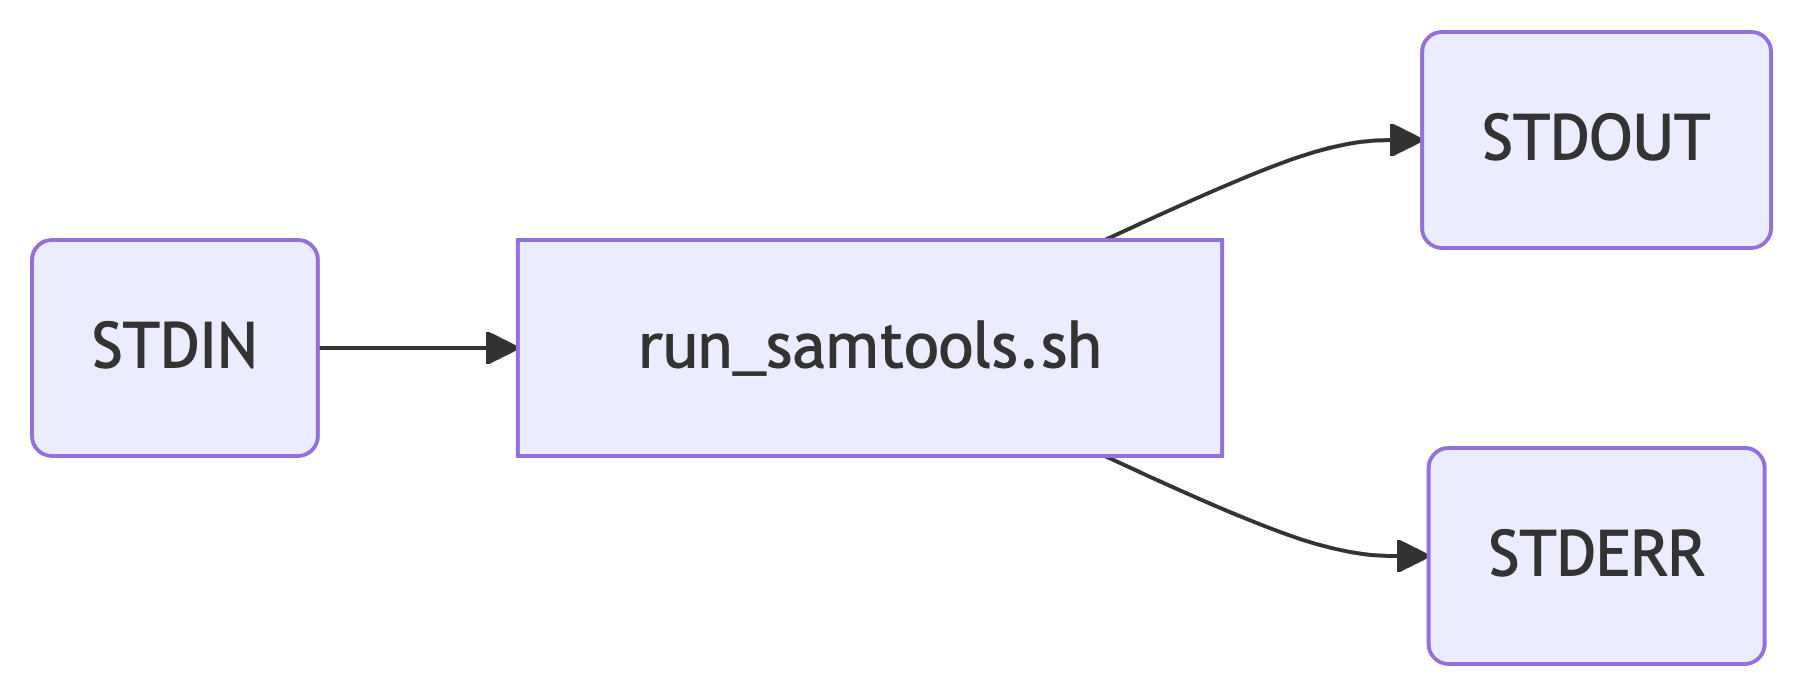
\includegraphics[width=3.58in,height=3.9in]{miscellaneous_files/figure-latex/mermaid-figure-4.png}

\section{Quoting and Escaping Filenames in
Bash}\label{quoting-and-escaping-filenames-in-bash}

One point of confusion is when do you quote things in Bash? When do you
use single quotes (\texttt{\textquotesingle{}}) versus double-quotes
(\texttt{"})? When do you use \texttt{\textbackslash{}} to escape
characters?

Let's talk about some quoting rules in Bash. I've tried to make things
as simplified and generalized as possible, rather than stating all of
the rules for each quote.

\begin{enumerate}
\def\labelenumi{\arabic{enumi}.}
\tightlist
\item
  If you have spaces in a filename, use double quotes
  (\texttt{"chr\ 1.bam"})
\item
  If you have a single quote in the filename, use double quotes to wrap
  it (\texttt{"ted\textquotesingle{}s\ file.bam"})
\item
  Only escape characters when necessary - if you can solve a problem
  with quotes, use them
\item
  If you need to preserve an escaped character, use single quotes
\end{enumerate}

Let's go over each of these with an example.

\subsection{If you have spaces in a filename, use double quotes (Most
common)}\label{if-you-have-spaces-in-a-filename-use-double-quotes-most-common}

For example, if your filename is \texttt{chr\ 1\ file.bam}, then use
double quotes in your argument

\begin{verbatim}
samtools view -c "chr 1 file.bam"
\end{verbatim}

\subsection{If you have a single quote in the name, use double quotes to
wrap it (less
common)}\label{if-you-have-a-single-quote-in-the-name-use-double-quotes-to-wrap-it-less-common}

Say you have a file called
\texttt{ted\textquotesingle{}s\ new\ file.bam}. This can be a problem
when you are calling it, especially because of the single quote.

In this case, you can do this:

\begin{verbatim}
samtools view -c "ted's new file.bam"
\end{verbatim}

\subsection{Only escape characters when necessary (less
common)}\label{only-escape-characters-when-necessary-less-common}

There are a number of special characters (such as Tab, and Newline) that
can be specified as escape characters. In double quotes, characters such
as \texttt{\$} are signals to Bash to expand or evaluate code.

Say that someone had a \texttt{\$} in their file name such as
\texttt{Thi\$file\ is\ money.bam}

How do we refer to it? We can escape the character with a backslash
\texttt{\textbackslash{}}:

\begin{verbatim}
samtools view -c "Thi\$file is money.bam"
\end{verbatim}

The backslash is a clue to Bash that we don't want variable expansion in
this case. Without it, bash would look for a variable called
\texttt{\$file}.

\subsection{If you need to preserve an escaped character, use single
quotes (least
common)}\label{if-you-need-to-preserve-an-escaped-character-use-single-quotes-least-common}

This is rarely used, but if you need to keep an escaped character in
your filename, you can use single quotes. Say we have a filename called
\texttt{Thi\textbackslash{}\$file.bam} and you need that backslash in
the file name (btw, please don't do this), you can use single quotes to
preserve that backslash:

\begin{verbatim}
samtools view -c 'Thi\$file.bam'
\end{verbatim}

Again, hopefully you won't need this.

\subsection{For More Info}\label{for-more-info}

\url{https://www.grymoire.com/Unix/Quote.html\#uh-3}

\begin{tcolorbox}[enhanced jigsaw, colbacktitle=quarto-callout-note-color!10!white, left=2mm, toprule=.15mm, toptitle=1mm, opacityback=0, bottomrule=.15mm, breakable, leftrule=.75mm, colframe=quarto-callout-note-color-frame, bottomtitle=1mm, titlerule=0mm, coltitle=black, title=\textcolor{quarto-callout-note-color}{\faInfo}\hspace{0.5em}{What about backticks?}, rightrule=.15mm, arc=.35mm, opacitybacktitle=0.6, colback=white]

Backticks (\texttt{\textasciigrave{}}) are an old way to do command
evaluation in Bash. For example, if we run the following on the
command-line:

\begin{verbatim}
echo "there are `ls -l | wc -l` files in this directory"
\end{verbatim}

Will produce:

\begin{verbatim}
there are       36 files in this directory
\end{verbatim}

Their use is deprecated, so you should be using \texttt{\$()} in your
command evaluations instead:

\begin{verbatim}
echo "there are $(ls -l | wc -l) files in this directory"
\end{verbatim}

\end{tcolorbox}

\begin{tcolorbox}[enhanced jigsaw, colbacktitle=quarto-callout-note-color!10!white, left=2mm, toprule=.15mm, toptitle=1mm, opacityback=0, bottomrule=.15mm, breakable, leftrule=.75mm, colframe=quarto-callout-note-color-frame, bottomtitle=1mm, titlerule=0mm, coltitle=black, title=\textcolor{quarto-callout-note-color}{\faInfo}\hspace{0.5em}{What about X use case?}, rightrule=.15mm, arc=.35mm, opacitybacktitle=0.6, colback=white]

There are a lot of rules for Bash variable expansion and quoting that I
don't cover here. I try to show you a way to do things that work in
multiple situations on the cluster.

That's why I focus on double quotes for filenames and \texttt{\$\{\}}
for variable expansion in general. They will work whether your Bash
script is on the command line or in an App, or in WDL.

\end{tcolorbox}

\section{Using pipes: STDIN, STDOUT,
STDERR}\label{using-pipes-stdin-stdout-stderr}

We will need to use pipes to chain our commands together. Specifically,
we need to take a command that generates a list of files on the cluster
shared filesystem, and then spawns individual jobs to process each file.
For this reason, understanding a little bit more about how pipes
(\texttt{\textbar{}}) work in Bash is helpful.

If we want to understand how to chain our scripts together into a
pipeline, it is helpful to know about the different streams that are
available to the utilities.

\begin{figure}

\centering{

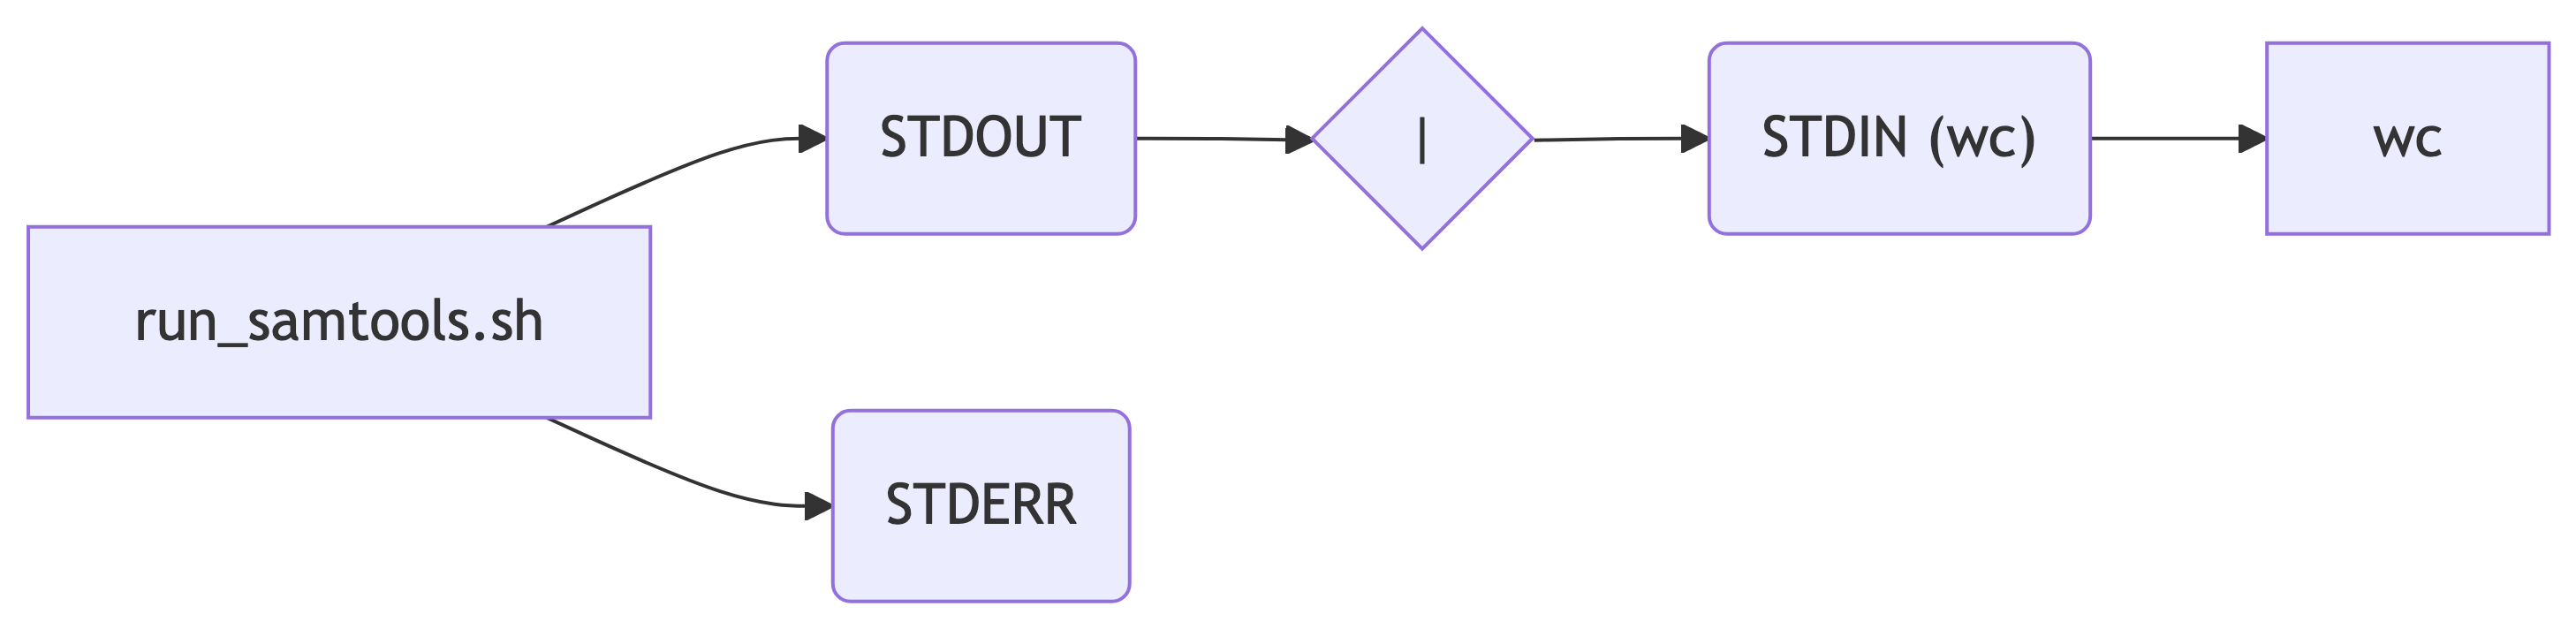
\includegraphics[width=4.7in,height=1.81in]{miscellaneous_files/figure-latex/mermaid-figure-3.png}

}

\caption{\label{fig-std}Inputs/outputs to a script}

\end{figure}%

Every script has three streams available to it: Standard In (STDIN),
Standard Out (STDOUT), and Standard Error (STDERR)
(Figure~\ref{fig-std}).

STDIN contains information that is directed to the input of a script
(usually text output via STDOUT from another script).

Why do these matter? To work in a Unix pipeline, a script must be able
to utilize STDIN, and generate STDOUT, and STDERR.

Specifically, in pipelines, STDOUT of a script (here it's
\texttt{run\_samtools}) is directed into STDIN of another command (here
\texttt{wc}, or word count)

\begin{figure}

\centering{

\includegraphics[width=7.6in,height=1.86in]{miscellaneous_files/figure-latex/mermaid-figure-2.png}

}

\caption{\label{fig-pipe}Piping a script \texttt{run\_samtools.sh} into
another command (\texttt{wc})}

\end{figure}%

We will mostly use STDOUT in our bash scripts, but STDERR can be really
helpful in debugging what's going wrong.

\begin{tcolorbox}[enhanced jigsaw, colbacktitle=quarto-callout-note-color!10!white, left=2mm, toprule=.15mm, toptitle=1mm, opacityback=0, bottomrule=.15mm, breakable, leftrule=.75mm, colframe=quarto-callout-note-color-frame, bottomtitle=1mm, titlerule=0mm, coltitle=black, title=\textcolor{quarto-callout-note-color}{\faInfo}\hspace{0.5em}{Why this is important on the Cluster}, rightrule=.15mm, arc=.35mm, opacitybacktitle=0.6, colback=white]

We'll use pipes and pipelines not only in starting a bunch of jobs using
batch scripting on our home computer, but also when we are processing
files within a job.

\end{tcolorbox}

\subsection{For more info about pipes and
pipelines}\label{for-more-info-about-pipes-and-pipelines}

\url{https://swcarpentry.github.io/shell-novice/04-pipefilter/index.html}
\url{https://datascienceatthecommandline.com/2e/chapter-2-getting-started.html?q=stdin\#combining-command-line-tools}

\section{\texorpdfstring{\texttt{basename} can be very handy when on
workers}{basename can be very handy when on workers}}\label{basename-can-be-very-handy-when-on-workers}

If we are processing a bunch of files on a worker, we need a way to get
the bare filename from a path. We will take advantage of this when we
run process multiple files on the worker.

For example:

\begin{verbatim}
basename /mnt/project/worker_scripts/srun-script.sh
\end{verbatim}

This will return:

\begin{verbatim}
srun-script.sh
\end{verbatim}

Which can be really handy when we name our outputs. This command is so
handy it is used in WDL.




\end{document}
